\documentclass[titlepage, 13px, a4paper]{report}

\usepackage[utf8]{inputenc}

\usepackage[T1]{fontenc}
\usepackage{fontawesome}
\usepackage{eurosym}

\usepackage[french]{babel}

\usepackage{fancyhdr}
\usepackage{graphicx}
\usepackage[left=4.5cm,right=4cm,top=4.5cm, textheight=17cm]{geometry}
\usepackage{wrapfig}

\usepackage{eso-pic}
\usepackage{transparent}

\usepackage{hyperref}
\usepackage{setspace}

\usepackage{titletoc}
\usepackage{titlesec}

\usepackage{stackengine,xcolor}
\usepackage{enumerate}

\titleclass{\part}{top}
\titleformat{\part}[display]
  {\normalfont\huge\bfseries}{\centering\partname\ \thepart}{20pt}{\Huge\centering}
\titlespacing*{\part}{0pt}{50pt}{40pt}
\titleclass{\chapter}{straight}
\titleformat{\chapter}[display]
  {\normalfont\huge\bfseries}{\chaptertitlename\ \thechapter}{20pt}{\Huge}
\titlespacing*{\chapter} {0pt}{50pt}{40pt}

%\usepackage{titlesec}
%\titleformat{\part}[display]
  %{\normalfont\bfseries}{}{0pt}{\Large\bfseries}

\newcommand\BackgroundPic{%
	\put(0,-50){%
		\parbox[b][\paperheight]{\paperwidth}{%
			%\vfill
			\centering
			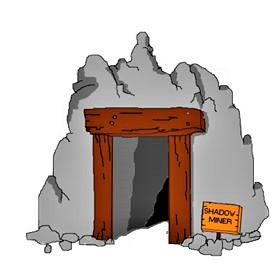
\includegraphics[%
			keepaspectratio]{../images/icone.jpg}%
			\vfill
		}
	}
}

\fboxrule=2pt
\newcommand\cincludegraphics[2][]{%
  \setbox0=\hbox{\includegraphics[#1]{#2}}%
  \abovebaseline[-.5\ht0]{\includegraphics[#1]{#2}}}

  
\renewcommand{\baselinestretch}{1}
\renewcommand{\partname}{}


\title{\textbf{{\Huge Manuel d'utilisation}}}
\author{
	\\
	\bsc{{\LARGE \bf ShadowMiner}} \\ \\ \\
	\bsc{{\LARGE \bf par ACCEr}} \\ \\
}
\date{{\LARGE \today}}

\pagestyle{fancy}
%\fancyfoot[L]{
\includegraphics{../images/ShadowMiners_logo_mini.png}} %50x33
\fancyfoot[L]{\cincludegraphics[scale=0.1]{../images/ShadowMiners_logo.png}} %50x33
\fancyfoot[R]{STRASBOURG 2022}
\fancyhead[R]{ACCEr}
\fancyhead[L]{Manuel d'utilisation}

\setcounter{tocdepth}{3}

\begin{document}
\AddToShipoutPicture*{\BackgroundPic}

\maketitle
\tableofcontents
%\listoftables
%\listoffigures

%################### INTRO

\fancypagestyle{plain}{}
\stepcounter{chapter}
\part{Introduction} 
\paragraph*{} \hspace{0pt}
Nous vous présentons notre rapport de projet. Ce dernier décrit l’état final du jeu ShadowMiner 
ainsi que tous ces composants. \\
Ce rapport de projet indique donc la sortie officielle du jeu ShadowMiner. \\

\paragraph*{} \hspace{0pt}
Après des mois de travail acharné, nous allons vous présenter ce que nous avons fait pour respecter 
notre cahier des charges et pour arriver à nos fins. \\

\paragraph*{} \hspace{0pt}
Nous allons tout d’abord vous présenter notre groupe : ACCEr. Puis nous allons décrire les 
principaux aspects du jeu ShadowMiner. \\

\paragraph*{} \hspace{0pt}
Ensuite chacun des membres du groupe décrira explicitement son travail effectué. \\
Enfin, nous indiquerons nos sources. \\

\paragraph*{} \hspace{0pt}
En bonus, nous avons rajouté quelques photos du jeu en annexe. \\

%################### INTRO


\newpage

%################### Qui sommes nous ?

\fancypagestyle{plain}{}
\stepcounter{chapter}
\part{Qui sommes-nous ?}
\section{Présentation des membres du groupe}

\paragraph{~~~~Cédric (Chef de projet)} \hspace{0pt} \\
Je m’appelle Cédric FARINAZZO. Je suis originaire de la région parisienne. 
A la suite des résultats du concours Advance, j'ai très rapidement accepté d'intégrer EPITA à Strasbourg. 
Malgré les contraintes géographiques, j'ai privilégié ma motivation pour suivre la formation à l'EPITA. 
Depuis, je me passionne pour l’informatique. J’adore découvrir de nouveaux langages ou me lancer des défis. \\
Réaliser un jeu vidéo est un rêve pour tout le monde. Ce projet est donc une occasion en or de le réaliser. 
Dès décembre, j’ai donc proposé à Clément et Antoine de faire ce projet ensemble, puis nous avons accueilli Edgar. \\
En tant que chef de projet, je donne donc le meilleur de moi-même afin de permettre la réussite de ce projet de groupe. \\


\paragraph{~~~~Antoine} \hspace{0pt} \\
Mon nom est Antoine (oui c'est aussi marqué juste au dessus en gras). 
J'ai commencé à apprécier les jeux vidéo lorsque mon père m'a fait découvrir la 
série de jeux « Half-Life ». Depuis j'ai exploré nombre mondes virtuels et j'ai 
continué à entretenir ma relation avec les jeux. Mon premier jeu vidéo, réalisé en 
groupe, fut un Snake codé en Python dans le cadre du projet d'ISN au lycée. C'est 
encore aujourd'hui un des meilleurs souvenirs que j'ai du lycée et j'étais donc bouillonnant 
à l'idée de pouvoir en créer un autre cette année à EPITA. Il n'a pas fallu beaucoup 
de temps pour que les grands esprits se rencontrent et j'ai rapidement sympathisé avec 
Cédric, puis Clément et enfin Edgar. Ensemble nous formons une équipe productive et 
inventive, et je suis content d'avoir pu réaliser ce projet avec eux. \\


\paragraph{~~~~Clément} \hspace{0pt} \\
Bonjour, je m'appelle Clément. J’ai grandi en région parisienne, à Antony. 
Je suis arrivé à EPITA par hasard, je m'étais renseigné sur l'école, le domaine de 
l'informatique m'a toujours beaucoup intéressé et je me suis retrouvé du jour au 
lendemain à Strasbourg, soit à 400 kilomètres de chez moi, livré à moi-même, avec 
ses avantages et ses inconvénients. \\
Heureusement, l'école et les cours m'ont tout de suite plu, ainsi que l'ambiance 
qu'il y a dans la classe. Je ne regrette pas du tout mon choix d'avoir intégré cette 
prestigieuse école dans cette magnifique ville qu'est Strasbourg. Ce projet est une 
réelle chance de pouvoir comprendre et apprendre comment les jeux vidéo fonctionnent, 
de comprendre certains "bugs" qu'on pouvait voir sur certains jeux.  \\

\newpage

\paragraph{~~~~Edgar} \hspace{0pt} \\
Je me présente : je m’appelle Edgar. J’ai commencé à m’intéresser vraiment à l’informatique  il y a trois ans . Je voulais 
vraiment savoir comment fonctionne tout ce que j’utilisais, même si plein d’autres choses m’intéressaient. Ce centre d’intérêt 
je pense qu’il me vient à l’origine des jeux vidéo. Aujourd’hui, je suis à Epita, je suis heureux de créer un jeu, notre jeu. 
C’est comme un accomplissement pour moi, j’avais envie de faire ça une fois dans ma vie. \\


\section{L'origine du nom du groupe : \textit{ACCEr}}
\paragraph*{} \hspace{0pt}
Le nom du groupe provient d’Antoine. A l’origine, nous nous appelions ACCer avant l’arrivée d’Edgar. 
« ACC » pour les initiales de nos prénoms et « er » pour porter confusion entre notre groupe 
et la société taïwanaise ACER, constructeur informatique bien connu. \\ \\
A l’arrivée d’Edgar, Nous avons décidé de mettre en majuscule le « e » de notre nom. \\
C’est ainsi qu’ACCEr est né.

\newpage

\section{Planning}
\paragraph*{} \hspace{0pt}
Voici un rappel de notre planning annoncé dans le cahier des charges : \\ \\
\\ \\
{
\begin{tabular}{|p{7.2cm}|p{1.2cm}|p{1.2cm}|p{1.2cm}|}
	\hline
	Pourcentages des tâches & \multicolumn{3}{|c|}{jusqu'à la soutenance} \\ 
	\cline{2-4}
		& \no 1 & \no 2 & \no 3 \\
	\hline
	Création des préfabs de map pour les niveaux (murs, sol, porte, ..) & 75\% & 100\% & 100\% \\
	\hline
	Modélisation 3D pour de meilleurs graphismes (si possible) & 0\% & 75\% & 100\% \\
	\hline
	Script c\# animation & 30\% & 60\% & 100\% \\
	\hline
	Création des préfabs des joueurs & 100\% & 100\% & 100\% \\
	\hline
	Script c\# joueur & 50\% & 75\% & 100\% \\
	\hline
	Création de multiples niveaux (entre 20 et 40) & 10-20\% & 50\% & 100\% \\
	\hline
	Création du Shadow Miner et Script c\# pour l'IA du Shadow Miner & 30\% & 60\% & 100\% \\
	\hline
	Cinématique du jeu & 0\% & 50\% & 100\% \\
	\hline
	Son du jeu & 0\% & 30\% & 100\% \\
	\hline
	Menu du jeu & 0\% & 40\% & 100\% \\
	\hline
	Création du site internet et Hébergement en ligne & 40\% & 80\% & 100\% \\
	\hline
	Création du serveur multijoueurs & 40\% & 90\% & 100\% \\
	\hline
	Création des joueurs pour multijoueurs & 30\% & 90\% & 100\% \\
	\hline
	Création du système de map aléatoire pour le multijoueurs & 0\% & 20\% & 100\% \\
	\hline
	Compilation du jeu et enregistrement sur CD & 0\% & 0\% & 100\% \\
	\hline 
	\end{tabular}
\label{Planning}	
}


%################### Qui sommes nous ?


\newpage

%################### ShadowMiner

\fancypagestyle{plain}{}
\stepcounter{chapter}
\part{Le jeu : ShadowMiner}
\section{Type de jeu et inspiration}
\paragraph*{} \hspace{0pt} \\
ShadowMiner est un jeu d’horreur dans une mine où évoluent un mineur et un monstre (le ShadowMiner). \\

\subsection{Inspiration}
Le jeu possède un mode solo et un mode multijoueurs, inspirés de différents jeux. \\
\paragraph[Inpiration du mode solo]{~~~~Inpiration du mode solo} \hspace{0pt} \\
Le mode solo est un "survival horror" imaginé à partir des jeux d'horreur du moment, 
en particulier "Outlast" et "Alien: Isolation" sortis en 2013 et 2014. 
\\
Le principe est de s'enfuir d'une mine en progressant dans une aventure guidée 
avec des «screamers» (moments de frissons/ frayeurs) prédéfinis et un scénario. 
Si le joueur n'est pas assez réactif, il peut mourir.
\\
Le terme "survival horror" fut utilisé pour la première fois en 1996 lors de la sortie 
de Resident Evil. Parmi les "survivals horror" les plus connus, nous pouvons citer "Outlast" qui 
nous a inspirés mais aussi "Until Dawn" et "Alien : Isolation". 
\\
Dans "Outlast", le joueur prend le contrôle d'un journaliste qui enquête sur un asile psychiatrique; 
"Until Dawn" raconte l'histoire d'un groupe de jeunes qui se rend dans un châlet 
en montagne pour passer les vacances. Le point fort de ce jeu réside dans son mode 
de jeu à la Heavy Rain ou Beyond Two Souls, c'est un film interactif dont l'histoire 
change radicalement en fonction des choix de l'utilisateur. 
\\
"Alien : Isolation" se déroule quatorze ans après les évènements du film "Alien, le huitième passager" 
et l'histoire est respectée dans les moindres détails. \\ \\

\paragraph[Inspiration du mode multijoueurs]{~~~~Inspiration du mode multijoueurs} \hspace{0pt} \\
Le mode multijoueurs est un "2 vs 1" dans le même genre que "Dead Realm", "Evolve" 
ou même "Mario Chase" dans Nintendo Land sur Wii U. 
\\
Dans "Dead Realm", trois joueurs se retrouvent dans un décor effrayant (vieux manoir, jardin de nuit, ...) enfermés 
avec un monstre terrifiant (loup garou, bébé tueur, clown) qui peut les transformer 
en spectre et s'en faire des alliés pour éliminer tous les survivants. 
\\
Dans "Evolve", quatre joueurs avec des compétences spécifiques se regroupent pour capturer 
une bête, mais elle devient plus forte au fil du temps et au final le chassé devient le chasseur. 
\\
"Mario Chase" est un mini jeu de cache-cache où un joueur possède une mini map 
avec la position de chaque joueur et doit réussir à ne pas se faire attraper par les autres. 
\\
Dans notre jeu, "ShadowMiner", un joueur incarne le ShadowMiner de la mine et les deux autres 
joueurs tentent de lui échapper. Parmi les deux mineurs il peut y avoir un esprit de la mine (explications ci-dessous). \\ \\


\section{Le mode solo}

\subsection[Scénario]{~~~~Scénario}
\paragraph*{} \hspace{0pt}
\begin{quotation}
	Un mineur descend tôt le matin dans les derniers sous-sols de la mine, là où l’oxygène se fait rare. 
	Un monstre (le Shadow Miner) coupe les câbles de l’ascenseur. 
	Le mineur veut alors rejoindre la surface. Le Shadow Miner va alors vouloir l’en empêcher. \\
\end{quotation}

\subsection[Gameplay]{~~~~Gameplay}
\paragraph*{} \hspace{0pt} \\
L’utilisateur incarne alors le mineur. \\
Le joueur devra donc progresser dans une série de niveaux de plus en plus difficiles. \\
Des pièges tels que des piques ou des trapes seront là pour le ralentir. \\
Le ShadowMiner lui-même sera là pour le traquer et le capturer dans les niveaux les plus difficiles. \\
Chaque niveau symbolise un étage de la mine. Le joueur devra donc rejoindre un checkpoint 
qui symbolise la fin d’un niveau, pour passer à l’étage suivant et donc au niveau suivant. \\
Le dernier niveau est ainsi la sortie de la mine. \\ 

\subsection[Progression du joueur]{~~~~Progression du joueur}
\paragraph*{} \hspace{0pt} \\
Le joueur devra réussir le niveau en cours pour accéder au niveau suivant. \\ \\
La progression du joueur est visible en jeu et sur le site internet \url{https://accer.ddns.net} si le joueur a lié son compte au jeu. \\

\newpage

\section{Le mode multijoueurs}

\subsection[Prérequis]{~~~~Prérequis}
\paragraph*{} \hspace{0pt} \\
Le joueur devra créer un compte pour pouvoir accéder au mode multijoueurs. \\
Ce compte pourra être créé sur le site internet \url{https://accer.ddns.net} ou dans le jeu lui-même. Ainsi le joueur pourra 
consulter et modifier ses données depuis le site internet \url{https://accer.ddns.net} ou depuis le jeu. Ce système lui permet 
de jouer sur n’importe quel exécutable du jeu en conservant ses données. 
Cela accroît fortement la portabilité du jeu. \\

\subsection[Gameplay]{~~~~Gameplay}
\paragraph*{} \hspace{0pt} \\
Le joueur rejoint tout d’abord un lobby, où il doit attendre que trois joueurs 
soient connectés avant que la partie ne commence.

\begin{figure}[h!]
  \centering
  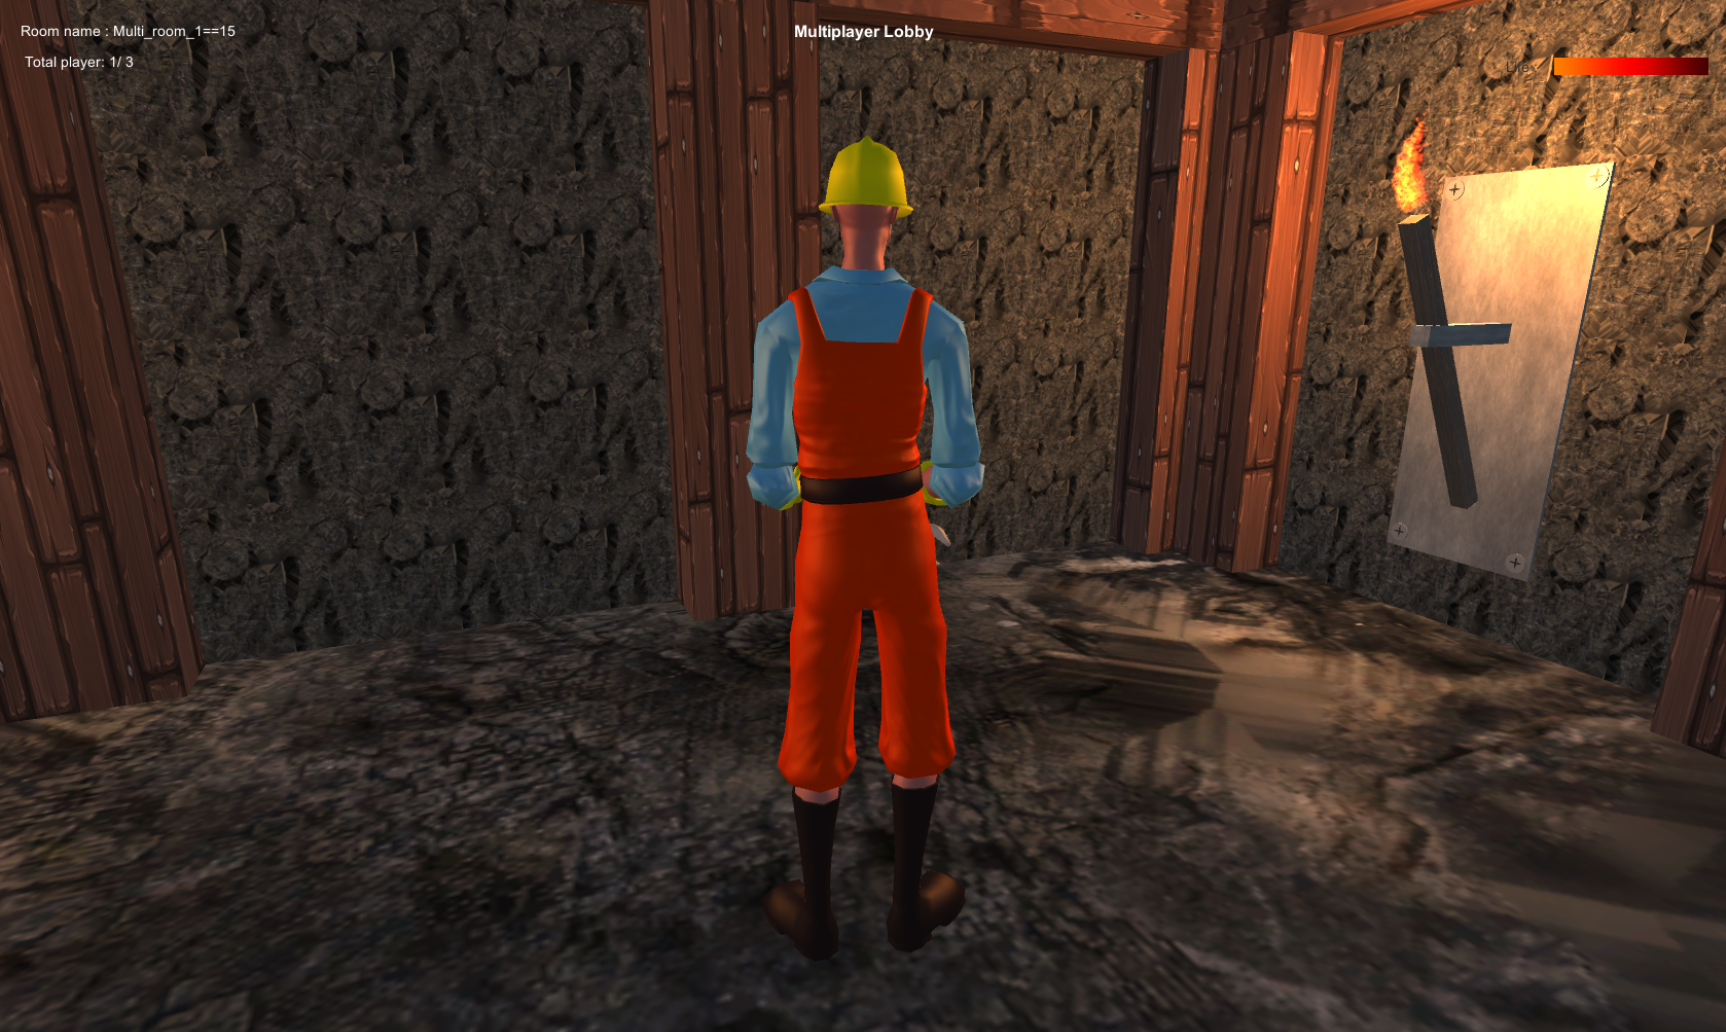
\includegraphics[scale=0.3]{images/multi_lobby.png}
  \caption{Le lobby du mode multijoueurs}
\end{figure}

\paragraph*{} \hspace{0pt} \\
Un joueur incarnera le ShadowMiner et devra tuer les deux autres joueurs qui 
incarneront deux mineurs voulant rejoindre la surface. Un des mineurs pourra 
s’enlever la vie et devenir un esprit de la mine, qui contrôle les cloisons de 
la mine (porte, mur, gouffre) pour aider l’autre mineur. \\

\paragraph*{~~~~Comment gagner ?} \hspace{0pt} \\
Deux solutions : \\
{\begin{itemize}
	\item Le ShadowMiner doit tuer tous les mineurs pour remporter la partie,
	\item Les mineurs doivent survivre jusqu’à la fin du minuteur pour remporter la partie. \\
\end{itemize}}

\subsection[Score du joueur]{~~~~Score du joueur}
\paragraph*{} \hspace{0pt} \\
Le joueur gagnera en score à chaque victoire en mode multijoueurs. \\
Son score sera visible en jeu mais aussi sur le site internet \url{https://accer.ddns.net}. \\
Un classement des meilleurs joueurs est d’ailleurs disponible sur le site internet \url{https://accer.ddns.net}. \\


\newpage

\section{Le site internet}
\subsection[Hébergement]{~~~~Hébergement}
\paragraph*{} \hspace{0pt} \\
L'adresse du site internet est \url{https://accer.ddns.net}. \\
Il est hébergé à Strasbourg chez Cédric sur un Raspberry Pi modèle 3B+. \\
L’accès au site est assuré par un élastique qui maintient le câble Ethernet relié au Raspberry pi. \\

\begin{figure}[h!]
  \centering
  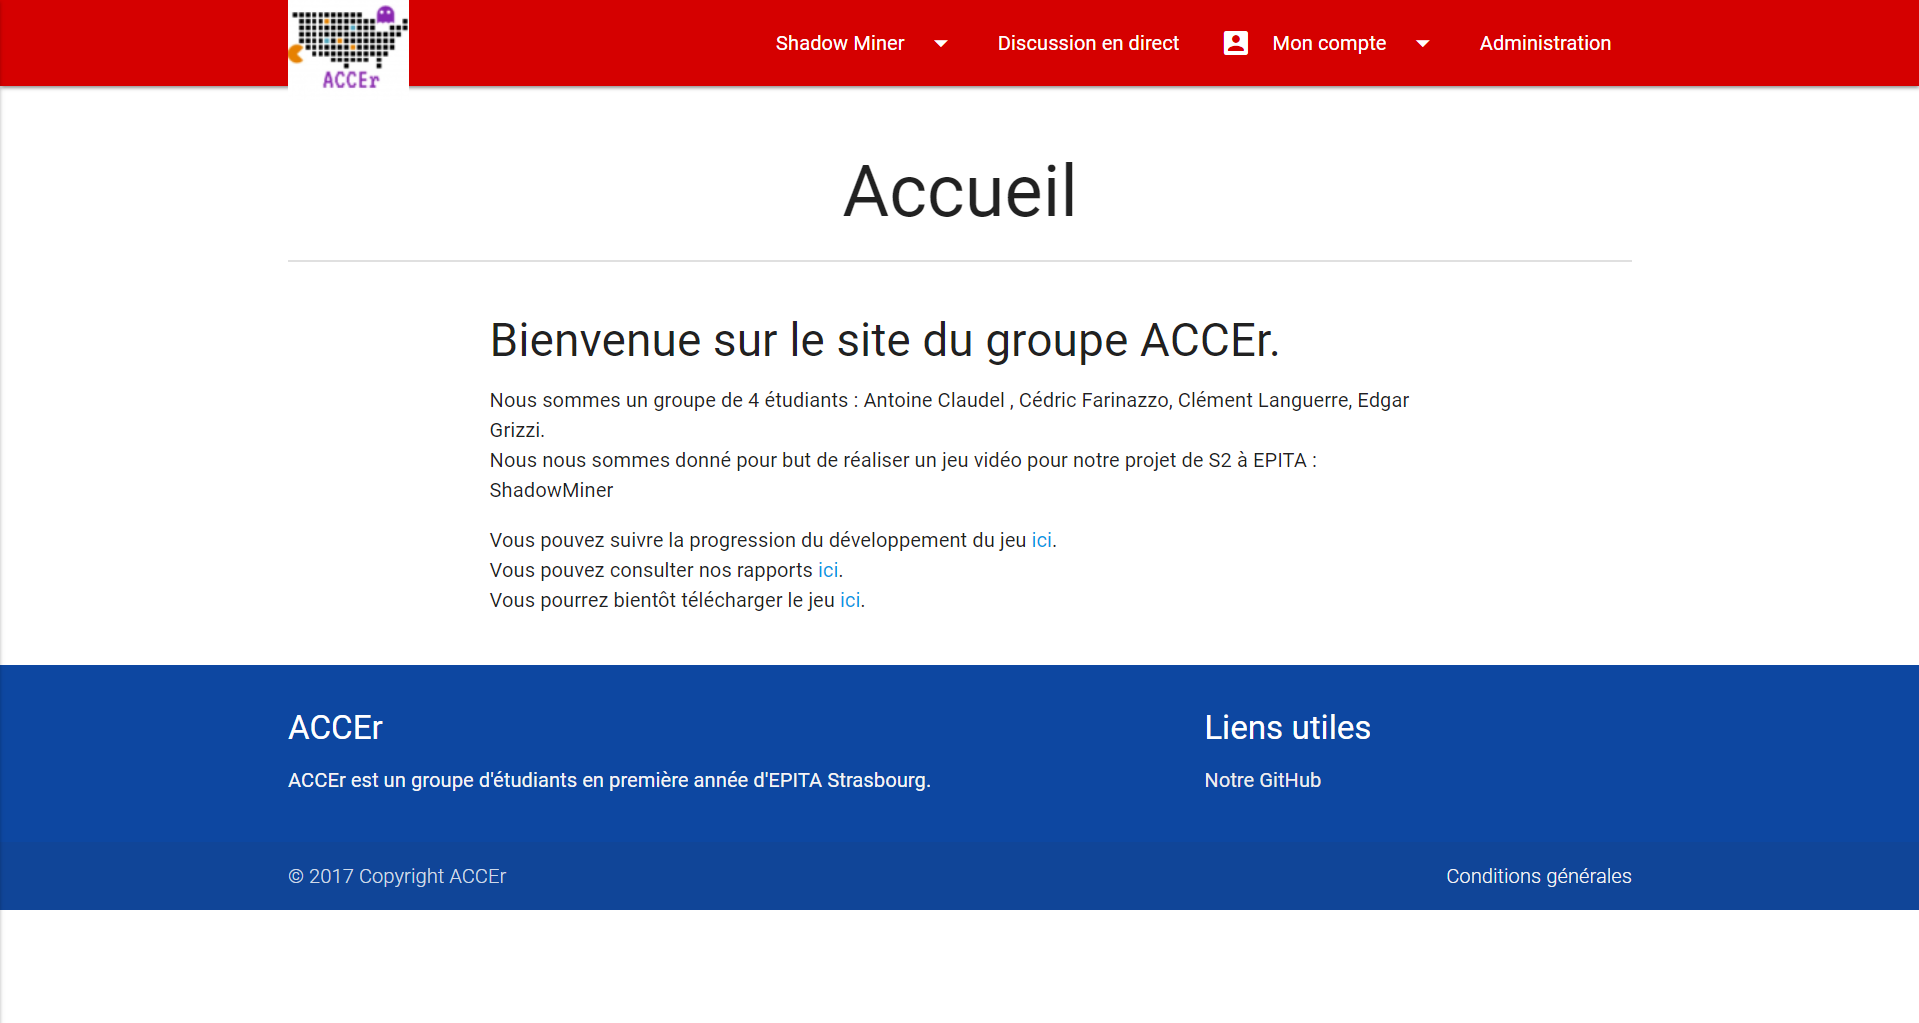
\includegraphics[scale=0.25]{images/website_accueil.png}
  \caption{L'accueil du site internet}
\end{figure}
\begin{figure}[h!]
  \centering
  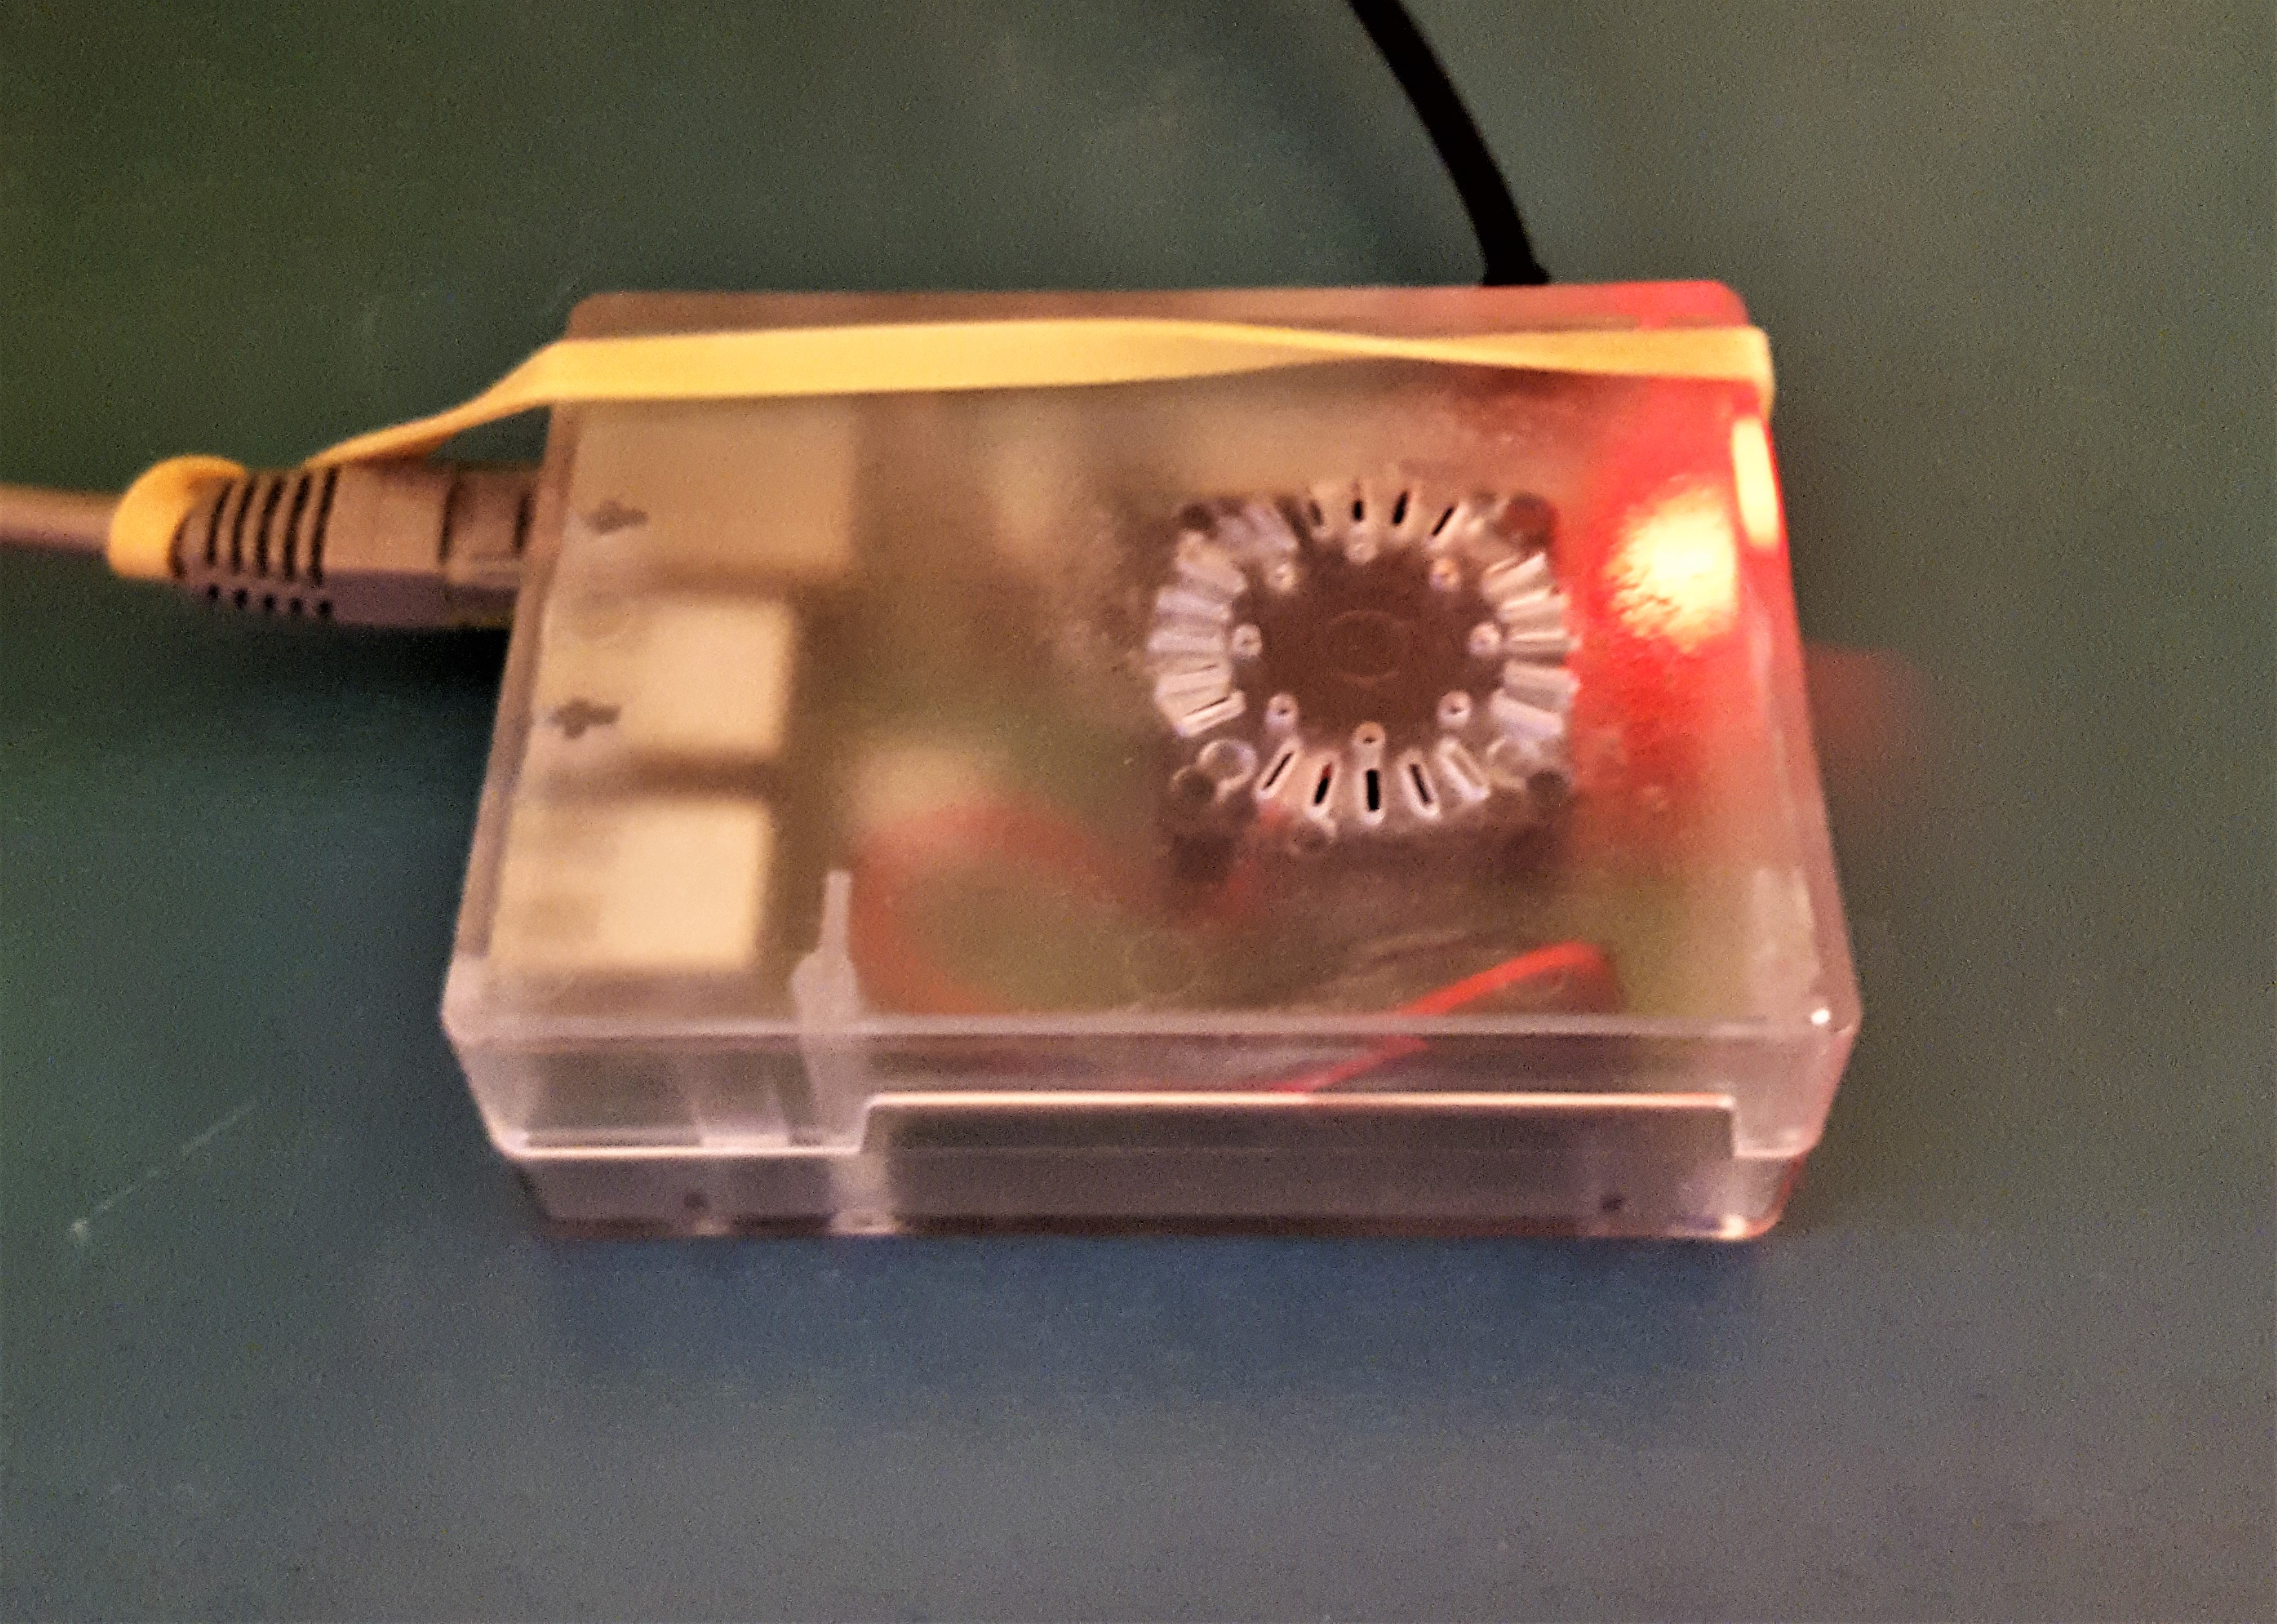
\includegraphics[scale=0.06]{images/website_rpi.jpg}
  \caption{Le Raspberry Pi}
\end{figure}

\newpage

\subsection[Compte]{~~~~Compte}
\paragraph*{} \hspace{0pt} \\
Le système de compte intégré au site internet \url{https://accer.ddns.net} permet de créer, 
gérer son compte comme par exemple, modifier son pseudo, sa description, son image de profil 
ou encore son mot de passe. \\

\subsection[L’onglet Shadow Miner]{~~~~L’onglet Shadow Miner}
\paragraph*{} \hspace{0pt} \\
Cet onglet permet d’accéder à plusieurs pages : \\
{\begin{itemize}
	\item Une brève description du projet (\url{https://accer.ddns.net/?p=project})
	\item Les sources utilisées (\url{https://accer.ddns.net/?p=source})
	\item La liste de tous les rapports (\url{https://accer.ddns.net/?p=report})
	\item Une page permettant de voir l’avancement du projet \\
		(\url{https://accer.ddns.net/?p=progress})
	\item Une page de téléchargement de l’installateur du jeu \\
		(\url{ https://accer.ddns.net/?p=download}) \\
\end{itemize}}

\subsection[Accès depuis le jeu]{~~~~Accès depuis le jeu}
\paragraph*{} \hspace{0pt} \\
Afin de pouvoir gérer son compte depuis le jeu, un serveur et un client ont été créés en C\#. \\
Le serveur écoute sur le port TCP 4247 (l’adresse est donc accer.ddns.net:4247). Ainsi le client, 
intégré au jeu, permet de créer un compte ou bien de se connecter, de modifier son pseudo, 
son mot de passe, sa description, son nom et son prénom. \\
Il permet aussi de synchroniser la progression du joueur en mode solo ou le score du joueur 
en mode multijoueurs (pour lequel il est obligatoire de créer un compte). \\

%################### ShadowMiner

\newpage

%################### Réalisation individuelle

\fancypagestyle{plain}{}
\stepcounter{chapter}
\part{Réalisations individuelles}
\section*{Introduction}
\paragraph*{} \hspace{0pt}
Nous allons maintenant vous présenter chacun à notre tour, le travail que nous avons réalisé, 
ainsi que ce que le projet nous a apporté. \\ \\

\section{Antoine}
\subsection{Introduction}
\paragraph*{} \hspace{0pt} 
Mes tâches pour ce projet furent la création des préfabs (objets complexes qui
serviront de base) pour les niveaux (murs, sol, porte, ..) et la création de multiples
niveaux. Elles ont été établies lors de la rédaction du cahier des charges début janvier. \\

\subsection{Description du travail}

\paragraph*{} \hspace{0pt} 
Pour débuter le projet j'ai commencé par construire des préfabs. Le tout premier
objet que j'ai utilisé est un cube 3D. En le dupliquant puis en assemblant ses
copies j'ai construit un mur en pierre. Ce fut le début de l'ère des préfabs. 
\begin{wrapfigure}{h!}{7cm}
  \centering
  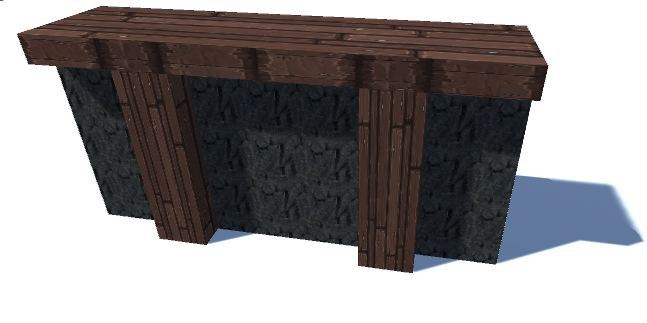
\includegraphics[width=7cm]{images/antoine_mur.png}
  \caption{Le mur}
\end{wrapfigure}
\\
Je construisis dans la foulée une table en bois. Les textures (bois et pierre)
proviennent d'un package gratuit de l'« asset-store ». Nous nous sommes ensuite
mis d'accord avec le groupe au sujet de cette plateforme : nous utiliserons le
moins possible son contenu comme l'exige le jury. \\

\paragraph*{} \hspace{0pt} 
Par la suite j'ai créé une flamme en utilisant le système de particule d'Unity3D, les
anciens élèves de 1ère année à EPITA nous avaient conseillés d'en abuser, car les
particules plaisent beaucoup aux professeurs. Mythe ou réalité ? Quoi qu'il en soit,
nous avons trouvé les flammes réussies et je m'en suis donc servi pour
confectionner des torches et des lanternes. J'avais donc respecté l'accord vis à vis
du contenu prémâché de l' «asset-store » d 'Unity3D. 

\newpage

\begin{wrapfigure}{h!}{7cm}
  \centering
  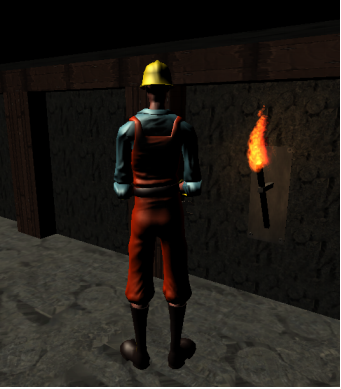
\includegraphics[width=7cm]{images/antoine_mineurtorche.png}
  \caption{La torche et le mineur}
\end{wrapfigure}

\paragraph*{} \hspace{0pt} 
Je continuais à le respecter en installant Blender. Ce logiciel m'a servi à créer des
rochers en modelant une sphère grâce à l'outil de sculpture. Après avoir transféré
les rochers sur Unity, j'ai ajouté un composant de gravité (Rigidbody) pour provoquer des
éboulements dans le jeu. Cette phase de création se situe peu avant la première
soutenance du 14 mars 2018. \\


\paragraph*{} \hspace{0pt} 
J'ai réalisé ma première interface utilisateur à ce moment. Il s'agit du premier menu
du jeu, composé de trois boutons : 1. Niveau un ; 2. Niveau deux ; 3. Multijoueur.
J'utilisais l'option « Add on click » d'Unity pour charger les scènes des trois niveaux
lorsque le joueur cliquait sur un bouton. Comme il n'y avait encore que trois
boutons, j'ai écrit un script (C\#) pour chaque bouton. Le niveau 1 fut construit par
Clément et la scène multijoueurs par Cédric. Je m'étais occupé du niveau 2. Ce
niveau commence dans un couloir peu éclairé (avec les murs construits
précédemment et quelques torches). Au bout du couloir sur la gauche, on trouve un
escalier condamné qui représente l'accès au niveau suivant. Le joueur doit donc
continuer à droite et après quelques pas, il se trouvera devant un énorme cratère
qui constitue la zone de minage. 
\begin{wrapfigure}{h!}{7cm}
  \centering
  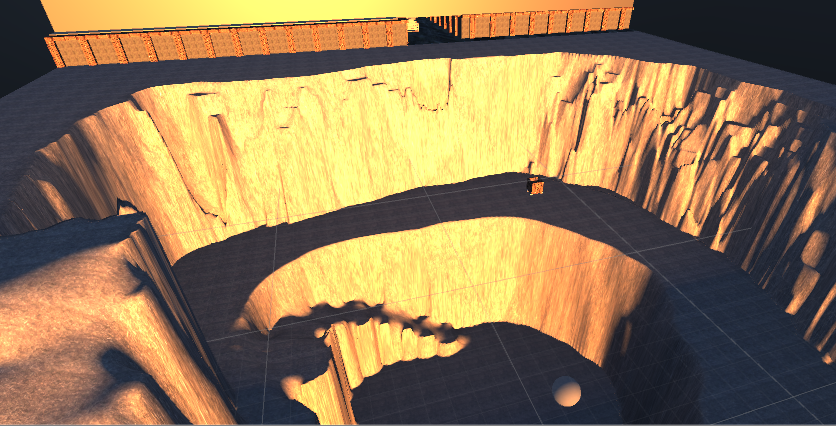
\includegraphics[width=7cm]{images/antoine_cratere.png}
  \caption{La zone de minage}
\end{wrapfigure}
\\

\paragraph*{} \hspace{0pt} 
Fin avril, la création d'autres niveaux commença. Je construisis un niveau avec un
sol qui s'écroule lorsque le joueur passe dessus et un niveau avec un passage
enflammé. A partir de ce moment, les flammes infligent des dégâts aux joueurs. Le
sol qui s'effondre et les flammes interagissent avec le mineur (personnage du
joueur) via leur « collider » (composant qui, en vulgarisant, permet de gérer les
collisions entre les objets). Ces niveaux atteignent leur objectif principal du point de vue de
l'originalité mais ils sont bien trop courts pour constituer des niveaux à eux seuls,
c'est pourquoi j'ai créé un grand niveau modèle qui a été dupliqué 19 fois. Les
deux mini-niveaux mentionnés ci-dessus ont donc été intégrés à deux des clones du
niveau modèle. \\


\paragraph*{} \hspace{0pt}
Le niveau modèle est un niveau assez simple sur le plan du gameplay mais plus
grand et plus impressionnant (si si, je vous assure). Il débute avec un couloir
comme les deux premiers niveaux construits avant la première soutenance mi-mars. 
Le couloir comporte devant une porte qui cache les toilettes. Il continue jusqu'à
la salle de détente avec tables, étagères, tabourets et un jukebox. Le jukebox
permet d'activer/désactiver la musique ambiante. Après cette salle, le couloir
reprend et se termine dans un espace de minage avec des cagettes de pépites
d'or et des murs pleins de minerais. 
\begin{wrapfigure}{h!}{7cm}
  \centering
  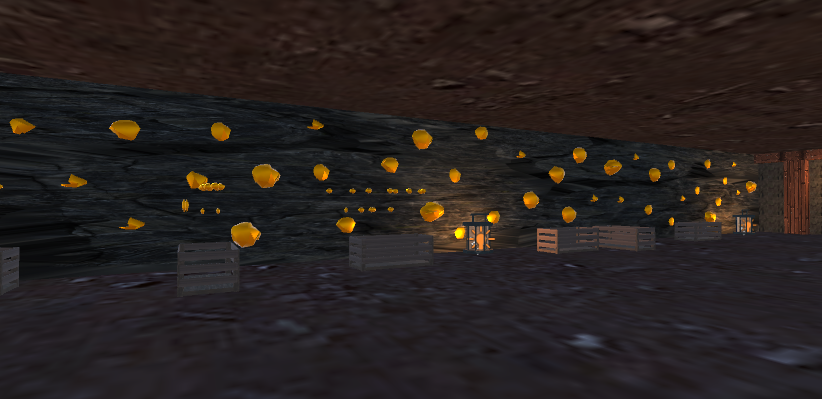
\includegraphics[width=7cm]{images/antoine_pepite.png}
  \caption{Les pépites}
\end{wrapfigure}
\\

\paragraph*{} \hspace{0pt} 
Dans le même temps, j'ai commencé la réalisation d'un niveau pour le mode
multijoueurs. Le plan du niveau a été réalisé sur Paint (logiciel de dessin) et ce
niveau contient un labyrinthe, des faux murs (qui se comportent comme des
portes), des passages sous-terrains et un pont tournant. \\
 
\paragraph*{} \hspace{0pt} 
Pour le menu du jeu, j'ai d'abord assemblé boutons et textes pour créer une
interface de connexion au serveur, puis d'inscription. J'ai ensuite repris la première
scène du choix des niveaux (avec les trois boutons rappelez-vous) et j'ai rajouté
les 17 autres niveaux (les clones du niveau modèle). 
\newpage
\begin{wrapfigure}{l}{7cm}
  \centering
  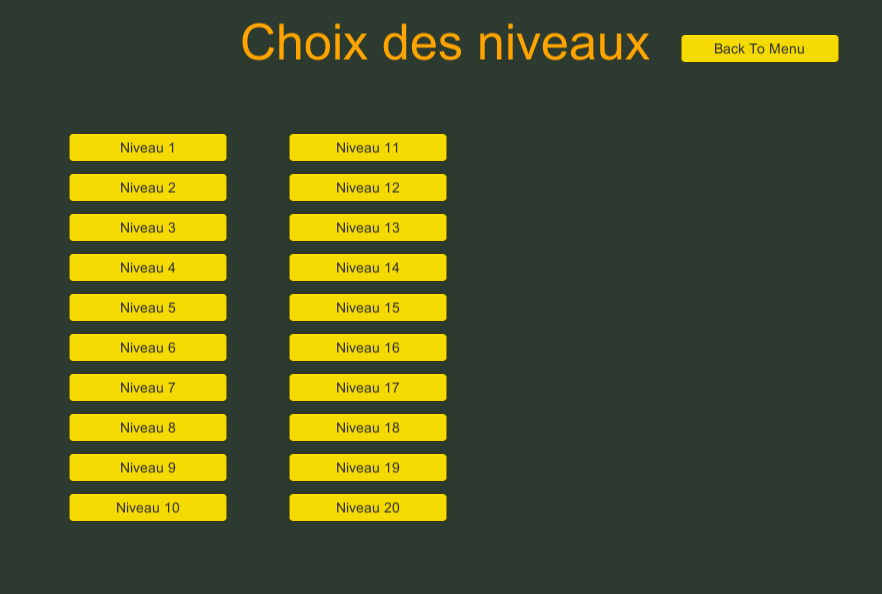
\includegraphics[width=7cm]{images/antoine_choixniveau.png}
  \caption{Le menu des niveaux solo}
\end{wrapfigure}

Cédric, étant responsable de la création du site internet \url{https://accer.ddns.net}, 
m'a aidé à utiliser le script qu'il avait créé permettant 
d'échanger des données avec le serveur et d'autres aspects du menu. Ainsi le script prend
en paramètre une liste des niveaux et des boutons et charge la scène adaptée
lorsqu'on clique sur un des boutons. Nous avons aussi créé la scène « mon
profil » qui permet à l'utilisateur d'accéder aux informations de son compte
(prénom, nom, adresse mail, mot de passe, description et pseudo) et de les
modifier. 
\begin{wrapfigure}{h!}{7cm}
  \centering
  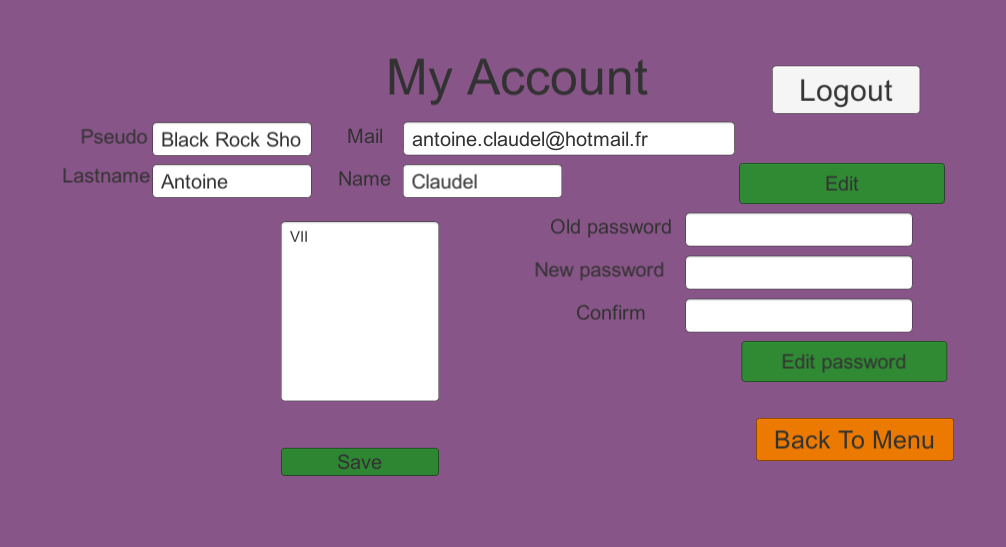
\includegraphics[width=7cm]{images/antoine_myaccount.png}
  \caption{Le menu des comptes}
\end{wrapfigure}
\\

\paragraph*{} \hspace{0pt} 
Pour terminer, ma dernière contribution au projet (avant la soutenance finale car je
prévois d'améliorer le jeu par la suite) fut de créer d'autres niveaux pour les
ajouter aux copies du terrain modèle et rendre chaque niveau différent. \\


\subsection{Apports personnels}
\paragraph*{} \hspace{0pt}
Ce projet m'a apporté énormément de choses, en particulier sur les plans techniques, 
organisationnels et humains. Pour commencer, réaliser un projet	
de plusieurs mois impose un temps de travail conséquent. Ce temps de travail est
d'autant plus optimisé qu'il est régulier, nous en avons fait l'expérience. J'ai donc
appris à mieux me rendre compte de mes capacités, à optimiser les heures avec le
groupe, les heures en salle machine et les heures de rêverie à imaginer les
prochaines étapes du projet. \\

\paragraph*{} \hspace{0pt}
Au fur et à mesure de l'avancement du projet, j'ai rencontré plusieurs difficultés.
Par exemple, mes scripts C\# qui ne prenaient pas de variables dans Unity, les
flammes qui ne faisaient aucun dégât au joueur ou encore les murs qui
tremblaient sur leur point d'intersection. L’intelligence collective du groupe nous 
a permis de trouver des solutions à des nombreux problèmes ainsi que des voies de contournement. \\

\paragraph*{} \hspace{0pt} 
De plus, nous avons pu partager nos connaissance et expériences personnelles et échanger des bonnes pratiques. 
Dans la partie précédente (Description du travail), j'ai témoigné avoir
utilisé l'utilitaire « add on click » d'Unity, alors que par la suite, Cédric m'a montré
que la fonction « Button.OnClick.addListener() » dans un script C\# faisait la même chose. Cela évitait de devoir
configurer les vingt boutons de niveaux pour le choix du terrain en mode solo. \\

\paragraph*{} \hspace{0pt} 
Ce jeu vidéo est une réalisation concrète résultat de nos efforts et de notre travail d’équipe. 
Nous pourrons continuer à y travailler durant notre temps libre (s’il nous en reste) 
et notre projet rejoindra sur Internet la grande famille des projets EPITA alimentée 
par les promotions précédentes (\url{https://2018.epita.eu/archive/index.php?thread-105.html}). 
Une pierre de plus à l’édifice. \\


\subsection{Conclusion d'Antoine}
\paragraph*{} \hspace{0pt}
Je suis fier d’avoir réalisé l’ensemble des tâches prévue. 
Le menu du jeu est opérationnel, les niveaux
sont au nombre de vingt (et un pour le mode multijoueurs). \\
J'ai beaucoup apprécié le travail en équipe et j'ai pu en 
apprendre davantage sur ses bénéfices et ses contraintes. \\


\newpage
\section{Cédric}
\subsection{Introduction}
\paragraph*{} \hspace{0pt}
Depuis la création du projet, je travaille sur de multiples travaux, tels que le site web ou le multijoueur. \\
Etant chef de projet, je me suis mis au maximum à la disposition des trois membres de notre équipe. \\


\subsection{Travail réalisé}
\paragraph{~~~~Site internet} \hspace{0pt} \\
Dès la fin du cahier des charges, je commence le site internet en PHP/HTML et je finalise le système de 
compte qui permet de s’authentifier sur le site.

Avant la première soutenance, je rajoute rapidement l’onglet ShadowMiner et quelques pages dénuées, pour 
le moment, de contenu mais qui seront vite remplies par la suite. Je m’empresse de trouver une solution pour héberger le 
site internet. Aucune offre ne nous correspond. Je trouve donc l’idée du Raspberry pi par hasard et ce fut chose faite.

Après cette soutenance, je rajoute un système d’administration permettant de ne plus toucher directement 
à la base de données pour rajouter un rapport et je rends possible l’installion du jeu, en rajoutant un 
installateur sur la page de téléchargement. Un système de cache et des optimisations au niveau du serveur 
sont ajoutés afin d’améliorer la vitesse de chargement du site internet (cette dernière est divisée par deux).

Avant la deuxième soutenance, je rajoute la possibilité au joueur d’éditer son pseudo, qui sera par la suite affiché 
au-dessus de la tête des joueurs en mode multijoueurs. \\


\paragraph{~~~~Les débuts sur Unity} \hspace{0pt}     \\
Après le cahier des charges, j’ai voulu commencer à travailler sous Unity. Ayant fait le TP bonus sur 
Unity proposé par les ACDC (et ayant revisionné cinq fois la conférence), j’avais donc une bonne base pour commencer.

J’ai donc créé le premier préfab : une porte.
A l’aide d’un assemblage de cubes et d’une texture type bois de l’asset store (les mêmes qu' Antoine), 
j’ai créé un encadrement puis la porte en elle-même. J’ai rajouté une animation d’ouverture et de fermeture 
sur la porte et un script qui joue ces animations, lorsqu’un joueur aux alentours appuie sur la touche « E ». \\

J’ai ensuite modélisé la mine vue de l’extérieur sous Unity.
J’ai ensuite travaillé sur le joueur (le mineur) : j’ai tout d’abord récupéré le modèle 3D des standards assets d’Unity 4.x 
qui est un mineur (donc génial pour notre projet). J’ai ensuite créé le script en C\# qui permet de déplacer 
notre joueur, aussi bien en première personne qu’en troisième personne. \\

\begin{figure}[h!]
  \centering
  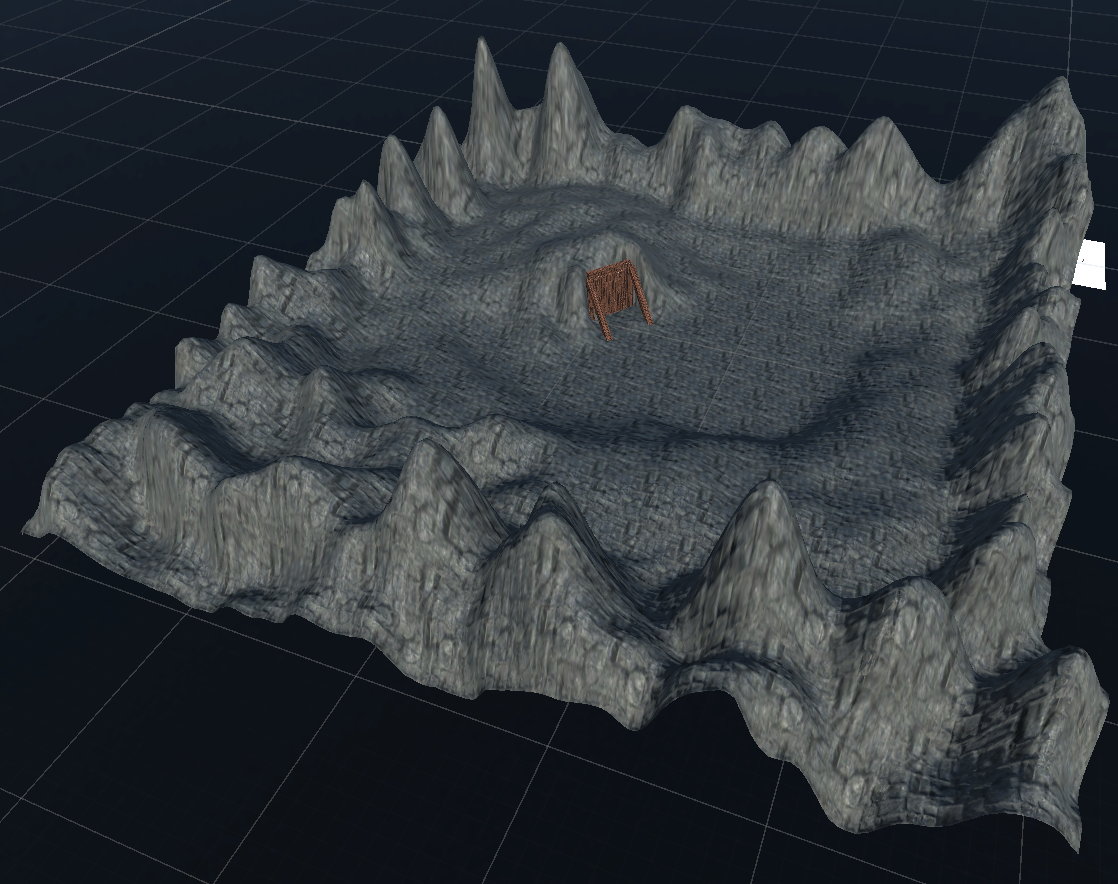
\includegraphics[scale=0.3]{images/cedric_mine.png}
  \caption{La mine vue de l'extérieur}
\end{figure}

\paragraph{~~~~Le multijoueur} \hspace{0pt} \\
Il nous avait été conseillé de présenter un début de multijoueur à la première soutenance. 
Je me suis donc occupé d’intégrer Photon Unity Networking (PUN) au projet.
Le script C\# nécessaire pour permettre le multijoueur était relativement simple.
Le multijoueur était donc opérationnel pour la première soutenance, mais il souffrait de quelques problèmes : \\
{\begin{itemize}
	 \item Les animations n’étaient pas synchronisées,
	 \item Les déplacements des autres joueurs n’étaient pas (voire pas du tout) fluides. \\
\end{itemize}}

Avant la deuxième soutenance, J'ai cherché et trouvé des solutions pour ces deux problèmes.
Pour les animations, il m’a fallu créer l’Animator Controller des animations du joueur et ajouter 
le composant Photon Animator View qui permet de retransmettre les valeurs des booléens (ou autres variables 
de l’Animator Controller) sur le réseau et donc de synchroniser les animations. \\

Pour le problème de fluidité, il suffisait de rajouter un composant Photon Transform View et d’utiliser la 
fonction Lerp (qui permet de modifier la position du joueur sans téléportation) de ce composant.

J’en ai profité pour rajouter un système de lobby. Une game est donc créée sur une map multijoueurs, choisie 
aléatoirement entre toutes les maps disponibles. Une game peut donc accueillir trois joueurs.

Lorsque les trois joueurs sont réunis, deux d'entre eux deviennent des mineurs et le dernier devient le ShadowMiner.
Tout le monde est ensuite téléporté dans la scène de jeu (il n’y a pas vraiment de changement de scène) et la partie commence.

Après la deuxième soutenance, j’ai rajouté : \\
{\begin{itemize}
	\item un écran de fin, permettant de savoir si le joueur a gagné,
	\item un minuteur qui accorde 3 minutes de temps de jeu.
	\item 2 autres maps multijoueurs pour rajouter de la diversité à ce mode. \\
\end{itemize}}

\paragraph{~~~~Accès au site depuis le jeu} \hspace{0pt} \\
Afin de rendre opérationnelles les scènes permettant de gérer son compte depuis le jeu créé par Antoine,
j’ai créé un serveur et un client en C\# communiquant sur le port TCP 4247. Le serveur étant lié à la même 
base de données MySql du site, les changements apportés sur nos comptes sont donc synchronisés avec les données du site internet.

Malheureusement, le serveur, qui se lance au démarrage du Raspberry pi, faisait monter le pourcentage 
du CPU utilisé, au point de ralentir le site internet.

J’ai donc utilisé la commande cpulimit (documentation : \url{https://doc.ubuntu-fr.org/cpulimit}) qui permet de donner une 
limite à un processus et donc de redonner de la vitesse de réponse au site internet. \\


\paragraph{~~~~Le menu des paramètres} \hspace{0pt} \\
Dès le début du projet, nous ne voulions pas du menu de démarrage d’Unity (le panneau de configuration avant 
le lancement du jeu qui permet de modifier les paramètres du jeu). Nous l’avons donc désactivé. \\

Mais un problème s’est posé : comment peut-on modifier les paramètres tels que la qualité des graphismes ou les touches sans ce menu ?
J’ai donc créé le menu des paramètres qui est composé de trois panels : \\
{\begin{itemize}
	\item Le panel Graphiques permettant de modifier la fréquence d’affichage, la qualité des graphismes, la résolution 
	de l’écran ou l’activation du mode plein écran,
	\item Le panel des touches permettant de changer la sensibilité de la souris ou de changer l’assignement des touches pour jouer,
	\item Le panel du son qui permet de modifier le volume sonore. \\
\end{itemize}}
A l’aide des PlayersPrefs (composants permettant de sauvegarder des données après la fermeture du jeu à l’aide de clé) 
et d’une classe Parametre créée pour l’occasion, ainsi que d’un petit coup de JSON sur une instance de la classe Parametre, 
les paramètres sont sauvegardés entre les différentes scènes. \\

\begin{figure}[h!]
  \centering
  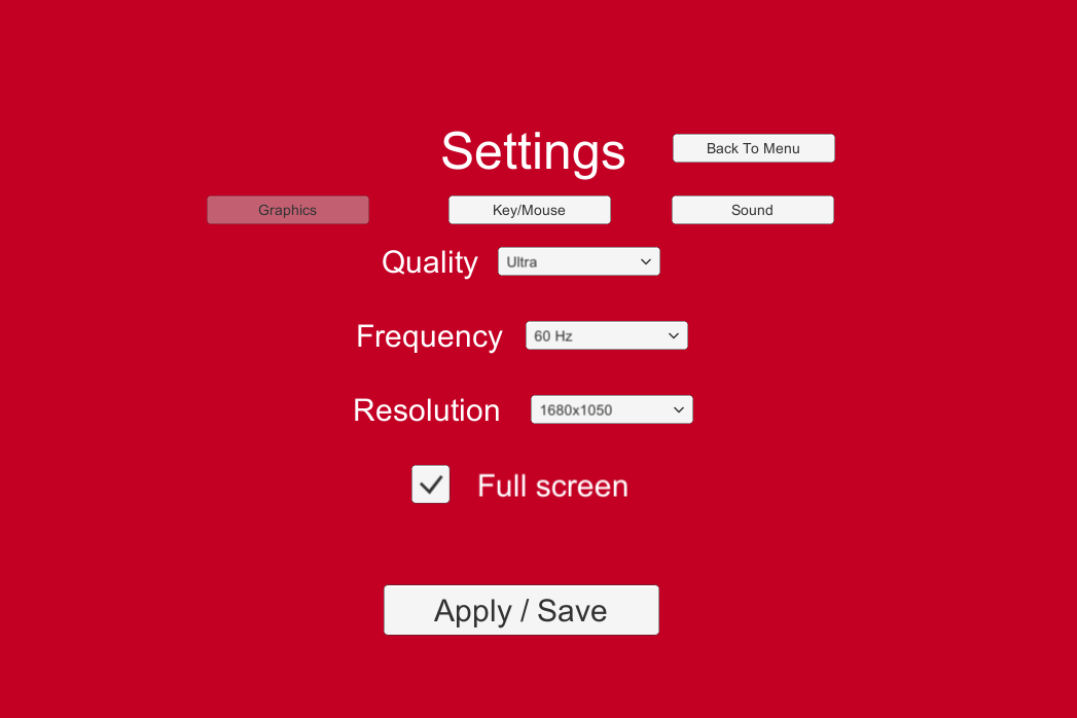
\includegraphics[scale=0.3]{images/cedric_parametre.png}
  \caption{Le menu des paramètres}
\end{figure}

\paragraph{~~~~La scène de chargement} \hspace{0pt} \\
Nous avions remarqué un ralentissement lors du chargement de certaines scènes particulièrement lourdes, nous avons donc eu 
l’idée de créer une scène de chargement qui chargerait les scènes.

A l’aide d’un bon tutoriel trouvé sur internet et de la méthode statique \textit{SceneManager.LoadSceneAsync}, cette scène 
de chargement était opérationnelle. \\


\paragraph{~~~~Le menu pause} \hspace{0pt} \\
Tous les jeux vidéo possèdent un menu pause : alors nous devions avoir le nôtre.
J’ai donc créé un préfab de ce menu qui est composé de deux boutons : \\
{\begin{itemize}
	\item Un bouton « Resume » qui permet de reprendre la partie,
	\item Un bouton “Back to menu” qui permet de revenir au menu principal. \\
\end{itemize}}
Le joueur peut donc mettre en pause le jeu en appuyant sur la touche « ECHAP » de son clavier. \\

\begin{figure}[h!]
  \centering
  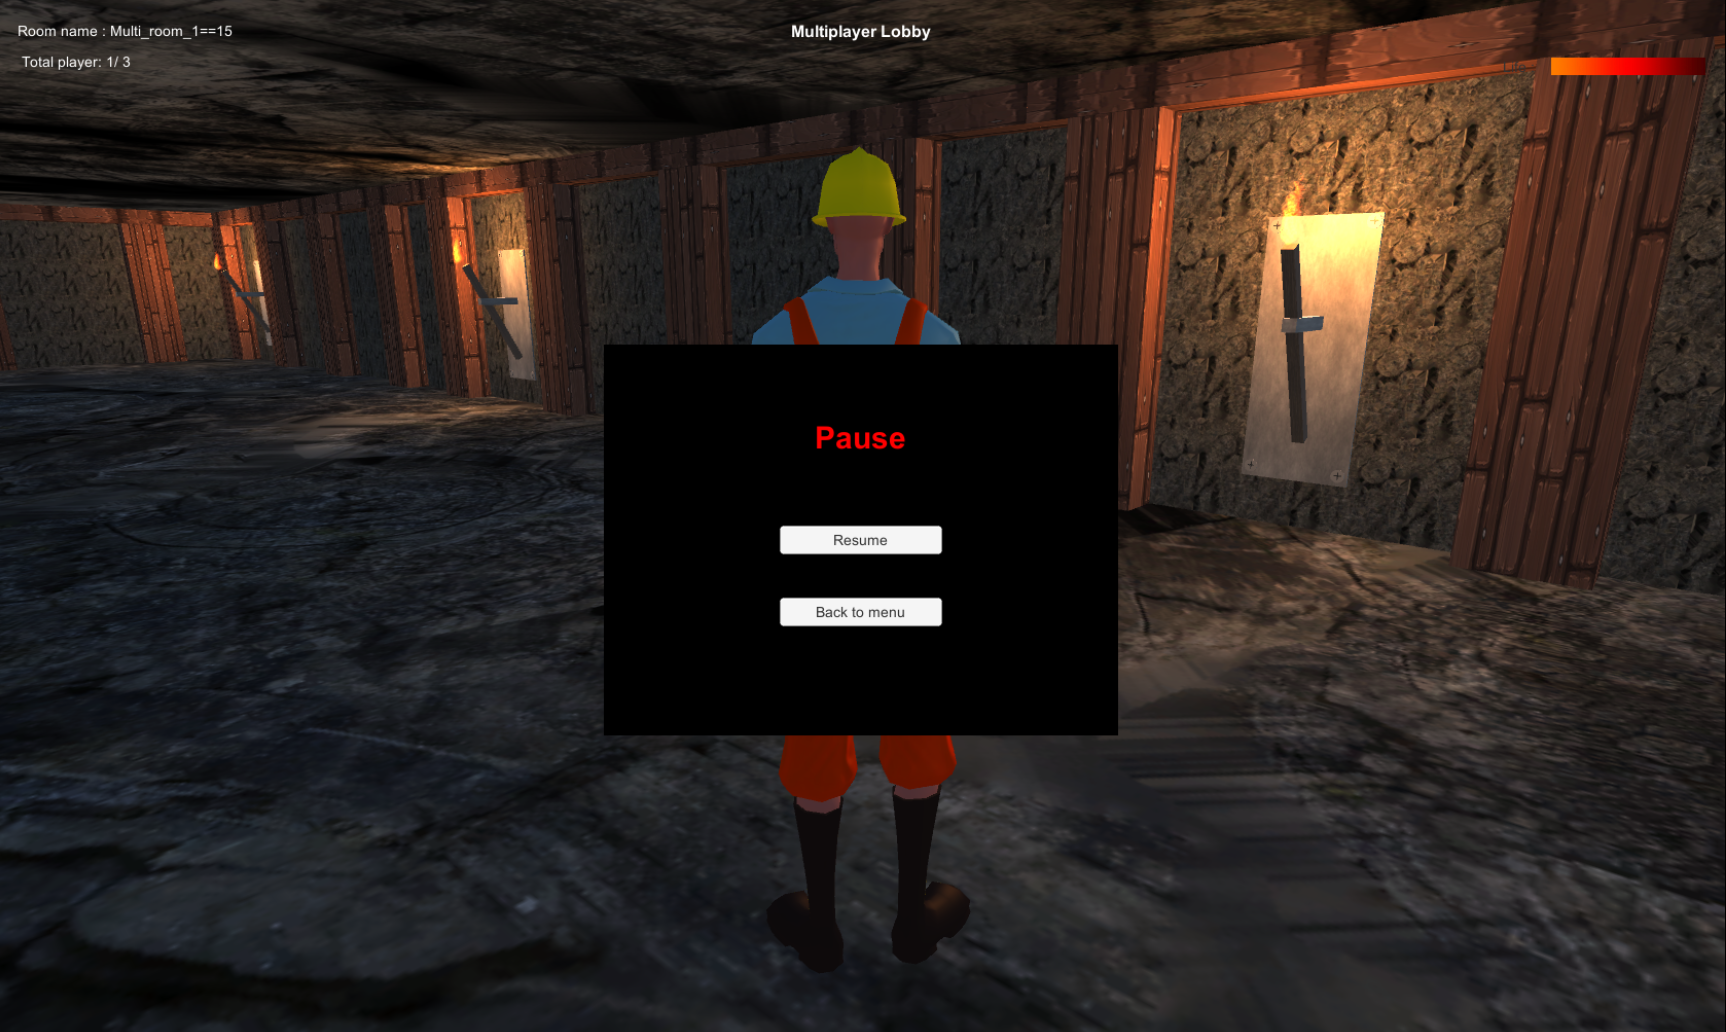
\includegraphics[scale=0.28]{images/cedric_pausemenu.png}
  \caption{Le menu de pause}
\end{figure}


\paragraph{\\ \\ \\~~~~Le ShadowMiner} \hspace{0pt} \\
\begin{figure}[h!]
  \centering
  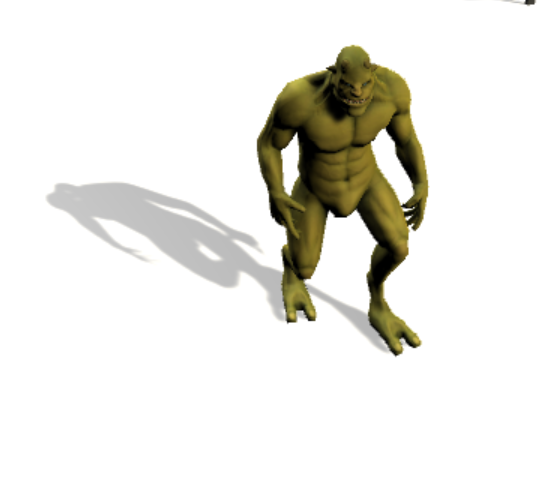
\includegraphics[scale=0.5]{images/cedric_shadowminer.png}
  \caption{Le ShadowMiner}
\end{figure}
Après quelques échecs avec les modèles 3D du ShadowMiner que nous avions trouvé pour la première soutenance, 
j’ai décidé de le remplacer par un monstre vert trouvé sur l’asset store.

J’ai ensuite créé l’Animator Controller de ce modèle 3D, afin de rendre possibles les animations.
J’ai ensuite utilisé le composant Nav Mesh Agent afin de rendre notre monstre « intelligent » en mode solo.
Il peut donc cibler un joueur si ce dernier passe trop près du monstre ou devant ce dernier. Il va ensuite le suivre et le tuer.
Pour le mode multijoueurs, il nous fallait un monstre qui puisse etre utilisé par le joueur.
Je lui ai donc rajouté un script permettant de le contrôler manuellement.
C’est ainsi que le multijoueur fut finalisé. \\


\paragraph{~~~~Editeur de map} \hspace{0pt} \\
Nous avions annoncé un système d’éditeur de map pouvant être créé par les joueurs.
N’ayant pas le temps de créer un tel système utilisable de façon correcte, nous avons utilisé le projet GILES 
disponible sur GitHub (\url{https://github.com/Unity-Technologies/giles}).

De ce fait, nous avons donc sérialisé l’objet obtenu. Ensuite la map sérialisée est envoyée au serveur et peut être 
jouable par n’importe quel joueur possédant un compte. \\


\subsection{Apports personnels}
\paragraph*{} \hspace{0pt}
Ce projet m’a beaucoup apporté dans deux domaines : \\
J’ai appris à gérer une équipe sur le long terme, à travailler et à m'adapter avec chacun des membres de l'équipe. 
Git nous a bien aidé pour mettre en commun nos travaux, malgré quelques merges à résoudre dont 
nous avions l’habitude au fil du temps. \\
L’équipe s’est renforcée et nous avons fait du bon travail du groupe. \\ 

\paragraph*{} \hspace{0pt}
Sur le plan technique, ce projet m’a permis de découvrir des technologies d’Unity telles que les Nav Mesh Agent 
pour l’IA ou encore Photon pour le multijoueur.
Mais ce projet nous a surtout appris à chercher par nous-mêmes les informations manquantes via la documentation 
très détaillée ou encore via des forums, sur lesquels d’autres personnes ont déjà rencontré 
et résolu les problèmes du même type que les nôtres. \\
Grâce à ces deux points, nous avons gagné en efficacité pour réaliser encore plus de fonctionnalités 
et enrichir notre projet. \\


\subsection{Conclusion de Cédric}
\paragraph*{} \hspace{0pt}
J’ai donc bien assumé mon rôle de chef de projet. J’ai rempli tous mes objectifs et 
j’en ai même fait plus que prévu. \\
Etant toujours très motivé, je compte continuer à développer ce jeu, même après la fin du projet en rajoutant du 
contenu et en fixant les nombreux bugs rapportés. \\


\newpage
\section{Clément}
\subsection{Introduction}
\paragraph*{} \hspace{0pt}
Lors de la formation des groupes, j'ai décidé de me mettre avec Cédric Farinazzo et Antoine Claudel 
pour former le groupe ACCer car je m'entendais bien avec eux et je savais que je pouvais rester 
sérieux en travaillant avec eux. On avait alors une idée de Battle Royale avec les gens de la 
classe combattant dans Strasbourg à l'aide de bretzel et de tartes flambés, plus communément 
appelé "flàmmenküeche". Avec l'arrivé d'Edgar Grizzi, nous nous sommes renommés ACCEr et nous 
avons opté pour un jeu Survival Horror dans une mine : Shadow Miner. \\

\subsection{Travail réalisé}
\paragraph*{} \hspace{0pt}
Nous nous sommes alors répartis les tâches selon ce que chacun voulait réaliser 
dans le projet. Personnellement, j'ai toujours aimé créer des maps et décorer 
des environnements à ma manière comme dans Super Smash Brawl, Brawl Stars ou encore 
Pokemon version Emeraude ; c'est pourquoi la tâche de la réalisation des différents 
niveaux m'allait parfaitement. N'ayant jamais utilisé Unity auparavant, j'ai d'abord 
regardé des tutoriels sur Youtube avant de commencer à l'utiliser. Je me suis aussi renseigné 
sur d'autres logiciels tels que Blender qui permet de faire des formes plus 
arrondies mais je le trouvais moins maniable qu'Unity. Je me suis d'abord exercé à créer des 
préfabs : chariot, étagère, table, chaises, poutre, obstacles, trousseau de clefs... \\

\paragraph*{} \hspace{0pt}
Avant de concevoir un niveau, je réfléchissais à la géométrique, à la structure et au 
mécanisme du niveau sur un tableau avant de travailler sur Unity. Ainsi, je savais ce 
que j'avais à faire dans le niveau. Pour le premier niveau, le joueur se retrouve au fin 
fond de la mine après que l'ascenseur se soit écrasé. Il doit alors quitter la mine en 
évitant les différents pièges et en ne se faisant pas tuer par le Shadow Miner, le monstre 
qui hante la mine. Le premier niveau est assez simple sans réelles difficultés à part le fait 
que ça soit un petit labyrinthe. Différents mécanismes sont implémentés comme le fait de 
pouvoir ouvrir une porte. \\

\begin{figure}[h!]
  \centering
  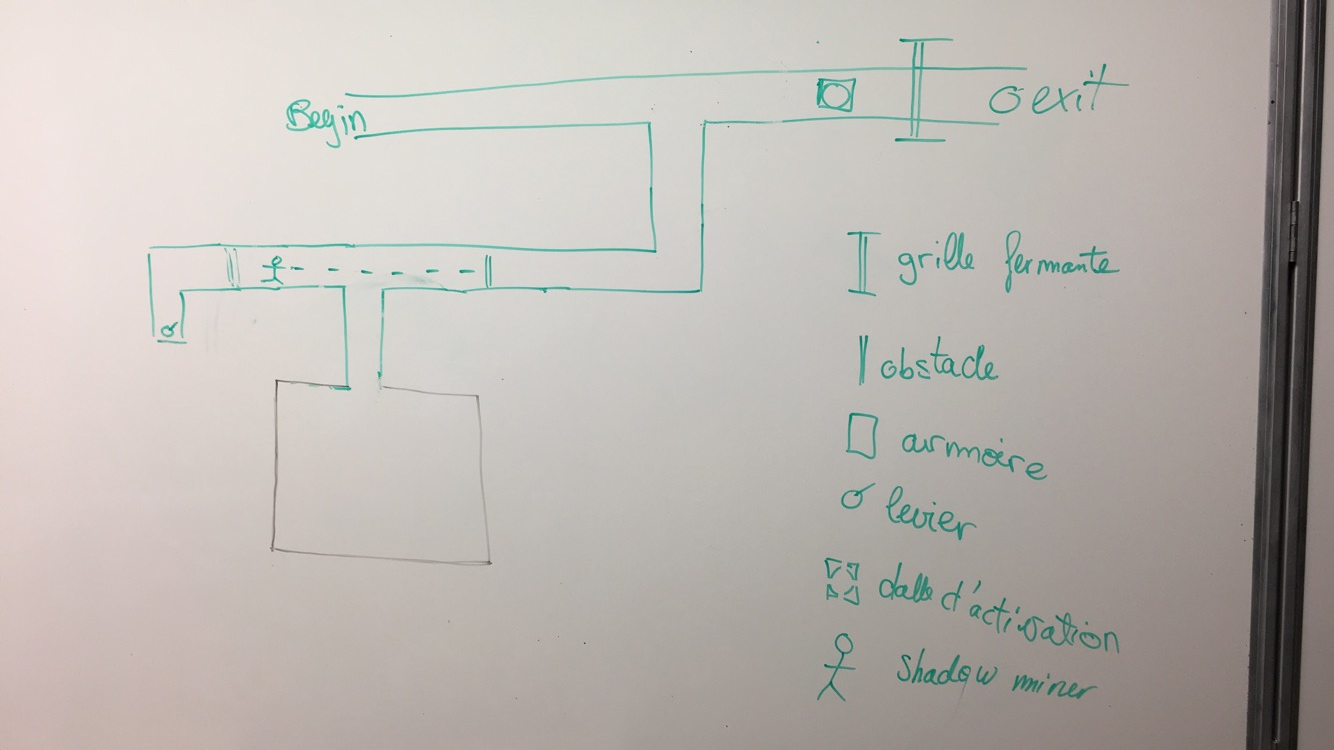
\includegraphics[scale=0.3]{images/clement_schema.png}
  \caption{Schéma d'un niveau réalisé par Clément}
\end{figure}

\newpage

\paragraph*{} \hspace{0pt}
Pour les niveaux suivants, je voulais que ces derniers soient plus compliqués, avec des 
objectifs à atteindre avant de terminer le niveau, un certain temps pour les accomplir. 
C'est pourquoi j'ai créé un préfab "grille" (dont je suis plutôt fier je l'avoue) pour bloquer 
le chemin du joueur. Cette grille peut s'ouvrir grâce à un levier qui se trouve à l'autre bout 
du niveau. Je trouvais ce niveau encore un peu trop facile, je voulais alors lui ajouter une autre 
difficulté, quoi de mieux que de rajouter le monstre de la mine : le Shadow Miner. La grille 
s'ouvre quand on active le levier (grâce à des scripts C\#).  \\

\begin{figure}[h!]
  \centering
  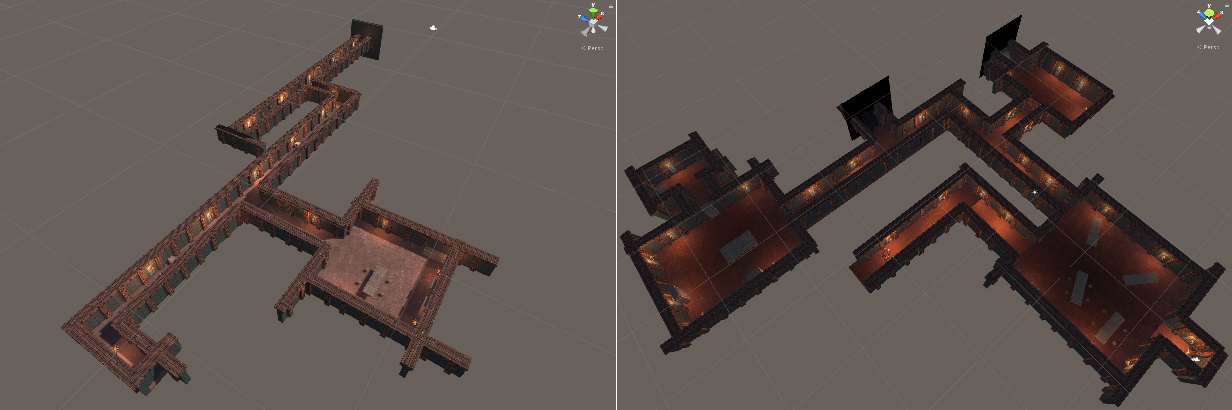
\includegraphics[scale=0.4]{images/clement_map_Final.png}
  \caption{Example de niveau réalisé par Clément}
\end{figure}

\paragraph*{} \hspace{0pt}
J'ai ajouté des cinématiques quand il y avait le Shadow Miner dans le niveau. 
Quand on actionne le levier, une cinématique nous montre ce qu'il se produit : une 
grille qui s'ouvre, un passage qui se débloque... je voulais aussi faire des cinématiques 
entre les niveaux un peu comme dans "The last of us" ou "Call of Duty", mais les graphismes 
d'Unity ne rendaient vraiment pas bien et je n'étais pas satisfait. \\

\subsection{Conclusion de Clément}
\paragraph*{} \hspace{0pt}
Notre groupe était bien soudé, chacun savait ce qu'il avait à faire. Je suis satisfait 
de ce que nous avons réalisé, j'ai pu apprendre beaucoup de choses, en cherchant sur 
Youtube comment réaliser quelque chose sur Unity ou grâce à mes équipiers de projet. 
Il y avait des séances de groupe qui nous permettaient de travailler ensemble, de demander 
l'avis de chacun des membres du groupe et les décisions pouvaient être prises très rapidement. 
Ce projet m'a permis de m'améliorer dans le travail en groupe, de découvrir de nouveaux 
logiciels et de comprendre ce qu'il se passait derrière la réalisation d'un jeu vidéo.  \

\newpage
\section{Edgar}

\subsection{Introduction}

\paragraph*{} \hspace{0pt}
Nous sommes en septembre, le projet est annoncé à toute la classe. 
J’étais déjà particulièrement enthousiaste avant, je connaissais l’existence du projet. 
En septembre, ma motivation pour le projet était plutôt haute, je commençais à avoir quelques idées 
qui me paraissaient sympathiques, bonnes, d’autres vraiment mauvaises. Dans mon coin, 
j’avais noté quelques idées possibles que je trouvais bonnes comme un logiciel avec plein de jeux de société, 
un jeu dans un endroit plutôt lugubre avec un monstre, un jeu de combat et quelques autres. 
Mon souhait était clairement de créer un jeu de toutes pièces avec mes camarades, 
je voulais voir et savoir comment créer quelque chose qui me paraissait complexe. 
L’aspect " construction"  était sûrement la chose la plus intéressante à ce moment où notre aventure 
n’avait pas encore commencé. En Octobre-Novembre, je commence à me chercher un groupe avec lequel je pourrais 
m’entendre et travailler, je cherchais un groupe qui pouvait avoir les qualités d’un bon groupe 
qui sont selon moi, l’entente, la communication, la notion de travail, l’organisation. 
La recherche de ce groupe fut complexe et vers décembre, un groupe se propose de m’accueillir, 
le groupe ACCEr était créé. Notre groupe était alors composé de Cédric Farinazzo, Antoine Claudel, 
Clément Languerre et de ma personne. Je ne me rappelle pas parfaitement si nous nous connaissions 
bien avant de venir en groupe, je connaissais un peu Cédric et Clément pour avoir fait 
la pré-rentrée avec eux, je n’ai aucun souvenir de bien connaître Antoine avant le projet. 
Aujourd’hui, je pense que nous nous connaissons plutôt bien. \\


\paragraph*{} \hspace{0pt}
Le nom du groupe est venu d'Antoine. Il avait mis les initiales de nos 
prénoms respectifs dans l’ordre alphabétique (ACCE), il rajouta alors un r minuscule pour 
que cela ressemble au constructeur informatique mondialement connu Acer. Nous n’avions pas 
d’autre idée, alors celle-ci fut retenue. Nous avons créé une conversation en groupe pour 
mieux communiquer, nous commençâmes à penser à notre idée de jeu chacun de notre côté et 
se dire nos idées principales pour le projet. Nous sommes en janvier, le projet démarre. 
Cédric propose une idée de jeu style Battle Royale, ce qui est particulièrement à la mode 
à ce moment de l’année. Clément propose un jeu dans une mine avec un monstre qui était une 
partie de mes idées, je trouvais cette idée excellente, selon moi c’était la meilleure idée, 
l’idée de ShadowMiner était née. \\

\subsection{Travail réalisé}

\paragraph*{} \hspace{0pt}
Notre aventure commence, le cahier des charges se fait dans les temps avec nos idées. Nous faisons une 
ou deux réunions de projet, où chacun de nous donne ses idées. Certaines idées vont un peu dans l'utopie 
pour un projet comme celui-ci, mais ces idées utopiques montrent quelque chose d'une importance cruciale 
voire vitale, nous étions motivés et enthousiastes. Un florilège d'idées sort de nos réunions. Nous avons 
alors choisi les meilleures selon nous et elles apparaissent aujourd'hui dans notre cahier des charges, 
même si certaines choses ont été modifiées depuis.  \\


\paragraph*{} \hspace{0pt}
Entre le début de la première soutenance, nous avons commencé le projet, pour moi un peu difficilement, 
je n'ai pas réussi à utiliser Unity à cause de mon ordinateur un peu vieux. \\
À présent je vais vous expliquer mon travail 
personnel sur le projet, où est-ce que j’ai œuvré à travers ce projet tout au long de l’année. \\


\paragraph*{} \hspace{0pt}
Avant la première soutenance, je me suis énormément concentré pour la modélisation 3D ainsi que le personnage 
du Shadow Miner, j’ai appris comment modéliser un personnage en 3D sur le logiciel Blender, 
cela m’a pris plusieurs heures pour avoir quelque chose que je trouvais pas si mal où je pouvais mettre 
des animations même si c’était un personnage sans visage, sans main et sans pied. J’avais créé un squelette 
en 3D qui pouvait recueillir des animations, ensuite je lui ai fait des muscles à ce personnage mais pour 
avoir un homme vraiment réaliste qui ressemble à quelque chose, je devais sûrement prendre un temps de travail 
considérable, peut-être dix fois plus que ce que j’avais mis dans la création de ce personnage en 3D. 
J’ai appris comment modélisé en 3D et cela m’a intéressé, donc j’étais content et heureux de l’avoir fait. 
Néanmoins, le travail fourni ne correspondait pas aux attentes de mes camarades en effet : il était particulièrement 
laid. \\ \\
C’était sûrement trop dur de créer un monstre 
ou un mineur donc nous sommes partis chercher des personnages de mineur et de monstres sur Internet dans des 
banques de données. Un camarade m’avait parlé du site Mixamo, je crois avoir passé quelques heures sur ce site 
pour l’analyser pour trouver des choses qui était bien pour le début de notre projet et avec Cédric nous avons 
trouvé le personnage et le physique de notre monstre (qui a été remplacé par la suite) et pour la soutenance, nous 
avons montré que nous pouvions déjà l’animer. Malheureusement, il était tout blanc. 
Quelques jours avant la première soutenance j’ai commencé utiliser à Unity sur un des ordinateurs du campus. 
Bien évidemment mes connaissances et mes compétences sur ce logiciel étaient totalement en retard par rapport à mes 
camarades, même si j’ai essayé de rattraper tant bien que mal ce retard. J’ai essayé de modéliser certaines 
choses sur Blender, telles que des roches, des amas de roches. En fait, tout était déjà fait mais aujourd’hui, 
j’ai appris à le faire et c’est cela le plus important. \\ \\
La première soutenance approchait à grands pas. 
La veille (et toute la nuit) Cédric et Clément ont fait un travail exceptionnel, que 
je me permet de souligné car ils ont œuvré comme des chefs pour obtenir un très bon résultat. \\

\paragraph*{} \hspace{0pt}
Pendant la période entre la première et la deuxième soutenance, 
nous avons fait du bon travail. Personnellement je me suis focalisé sur 
le son du jeu, parce que c’est quelque chose qui m’intéresse énormément, je voulais absolument enregistrer 
des sons ou aller en prendre sur des banques de données en ligne, pouvoir les modifier pouvoir avoir une 
musique de fond qui était bien pour le jeu. L’aspect sonore et audio du projet était sûrement 
la chose qui m’intéressait le plus. Pendant quelques jours, j’ai cherché des sons qui étaient idéaux pour le jeu, 
comme le bruit d’un éboulement de cailloux dans la mine, le cri du monstre, les bruits de pas, les bruits de cours. \\ \\
J’ai fait une dernière chose sur le son qui était les musiques de fond. 
Lors de notre première soutenance, pour montrer que nous pouvions mettre de la 
musique nous avions mis une musique qui rendait bien mais qui était particulièrement énervante au bout de 30 secondes 
d’écoute. Il nous fallait absolument une voire deux autres musiques de fond. C’est un ami du nom de 
Nicolas Masciocchi, que nous remercions particulièrement, qui a composé une musique. C’était une musique 
qui collait parfaitement bien avec certains temps, plutôt calmes avec du piano, et d’autres temps très puissant 
avec des cuivres et des violons qui peuvent très bien rendre le jeu plus vivant. J’ai découpé la musique en 
quelques parties évidemment, je garde l’original précieusement. L’aspect musical et sonore du jeu m’a fait 
comprendre à quel point le son est important dans un jeu. L’immersion est beaucoup plus présente et grâce à 
cette musique, le jeu en devient plus puissant et c’est une excellente chose pour nous. \\ \\
Cette fois-ci, nous avons vraiment bien travaillé et bien communiqué. Nous avions un travail qui était bon à mes yeux. 
Le rapport et le plan de soutenance ont été faits dans les temps, nous n’avions pas de retard. J’ai fait aussi avec 
Antoine le PowerPoint de la présentation, puis nous l’avons tous un peu modifié et cette fois-ci, nous étions vraiment 
prêts et préparés pour la deuxième soutenance et elle s’est très bien passée. Nous avons pu montrer le fruit de notre 
travail, notre projet n’était pas encore terminé mais, vu le travail déjà accompli, nous étions plutôt fiers. \\

\subsection{Conclusion d'Edgar}
\paragraph*{} \hspace{0pt}
Et aujourd’hui, nous écrivons notre rapport de projet. Cela nous rappelle et remémore des souvenirs de travail et 
de groupe. Certains moments furent stressants comme la préparation avant les soutenances, 
d’autres agréables comme des moments de rigolade dans le groupe, où nous blaguions entre nous. Le groupe 
ACCEr a fait son projet avec envie à mes yeux, en tous cas, c’est mon cas. je suis resté motivé pour ce projet, 
j’ai appris plein de choses très intéressantes pas forcément sur le plan informatique mais aussi sur le plan 
personnel. J’ai appris à communiquer dans un groupe que je ne connaissais que très peu. Aujourd’hui, j’aime 
travailler avec ses trois messieurs qui m’entourent. Nous espérons avoir fait un travail qui peut convenir 
au jury et nous espérons aussi répondre à leurs attentes. 

\newpage

\section*{Conclusion des réalisations individuelles}
\paragraph*{} \hspace{0pt}
Nous pouvons donc conclure que chacun a rempli ses objectifs.
Ce projet nous a beaucoup apporté et nous a appris à travailler en groupe et faire face à certains aléas.


%################### Réalisation individuelle

\newpage

%################### Sources et remerciements

\fancypagestyle{plain}{}
\stepcounter{chapter}
\part{Sources et remerciements}

\section{Sources}
\paragraph*{} \hspace{0pt}
N'étant pas des experts en modélisation 3D , nous avons dû trouver nos personnages sur internet : 
{\begin{itemize}
	\item Le mineur provient des standarts assets de Unity 4.x, nous avons juste récupéré le modèle 3D et les animations,	
	car nous n'avons pas le droit de récupérer de script. De plus, les scripts de l'asset étaient en Javascript(Unityscript).
	\item les textures sur les objets et les sols et le modèle 3D du ShadowMiner proviennent de 
		l'Assets Store.
	\item (\url{https://github.com/Unity-Technologies/giles}) pour la création de l'éditeur de map. \\
\end{itemize}} 

Voici aussi les sources des musiques et des effets sonores du jeu : \\
{\begin{itemize}
	\item \url{http://www.universal-soundbank.com/bruitdepas.htm}
	\item \url{http://www.universal-soundbank.com/terre.htm}
	\item \url{http://www.universal-soundbank.com/cris.htm} \\
\end{itemize}} 

\section{Technologies utilisées}
\paragraph*{} \hspace{0pt}
Pour réaliser ce projet, nous avons dû coder dans plusieurs langages et utiliser différentes technologies : 
{\begin{itemize}
	\item Unity3D, pour le moteur de jeu,
	\item Photon Unity Networking afin de mettre en place le mode multijoueurs,
	\item Git et Github afin de mettre en commum notre travail,
	\item C\# pour le jeu, 
	\item HTML, CSS, JavaScript, PHP, MYSQL pour le site internet,
	\item \LaTeX ~ pour les rapports. \\
\end{itemize}}

\paragraph*{} \hspace{0pt}
Nous avons aussi utilisé quelques Frameworks  afin de réaliser rapidement le design du site internet :
{\begin{itemize}
	\item Le framework JQuery (\url{https://jquery.com/}). pour simplifier la mise en place du javascript,
	\item Materialize css (\url{https://materializecss.com/}) permettant simplement de donner un style au site. \\
\end{itemize}}

\section{Remerciements}
\paragraph*{} \hspace{0pt}
Nous remercions Monsieur Nicolas Masciocchi pour nous avoir aimablement autorisé à utiliser sa musique 
comme musique de fond. \\

%################### Sources et remerciements

\newpage

%################### Conclusion

\fancypagestyle{plain}{}
\stepcounter{chapter}
\part{Conclusion}
\paragraph*{} \hspace{0pt}
Après la création du groupe ACCEr, nous nous sommes rapidement mis d’accord sur un jeu 
d’horreur dans une mine : ShadowMiner. \\

\paragraph*{} \hspace{0pt}
Ce projet nous a forcés à travailler dur pour atteindre nos objectifs et nous a appris à 
travailler en groupe et à utiliser des technologies dont nous ne connaissions pas, pour la 
plupart, l’existence avant le début du projet. \\

\paragraph*{} \hspace{0pt}
Notre groupe étant soudé, nous avons pu remplir les objectifs annoncés dans le cahier des 
charges de janvier et ainsi permettre la sortie officielle du jeu ShadowMiner. \\

\paragraph*{} \hspace{0pt}
Cependant, nous n’allons pas nous arrêter là : nous allons continuer de fixer les bugs 
et de rajouter du contenu à notre jeu. \\


%################### Conclusion

\newpage

\newpage

%################### Annexe

\fancypagestyle{plain}{}
\stepcounter{chapter}
\part{Annexe}
\paragraph*{} \hspace{0pt}
Voici quelques images du jeu : \\ \\


%################### Annexe

%################### Glossaire

\fancypagestyle{plain}{}
\stepcounter{chapter}
\part{Glossaire}
\paragraph*{} \hspace{0pt}
{\begin{enumerate}[I.]
	\item Unity : (également appelé Unity3D) moteur de développement de jeux-vidéo. \\
	
	\item Préfabs : objets complexes d'Unity permettant de créer des références 
	entres plusieurs objets. \\
	
	\item Collider : composant permettant de gérer les collisions avec d'autres objets 
	possédant ce composant.    \\

	\item Snake : jeu vidéo dans lequel le joueur dirige un serpend qui grandit et constitue 
	ainsi elle-même un obstacle.        \\

	\item Paint : logiciel d'édition et de création d'images de Microsoft.    \\

	\item Site web : Le site web du projet : \url{https://accer.ddns.net}.    \\

	\item Photon Unity Networking (PUN) : un service permettant de mettre en 
	place du multijoueur dans Unity. \\

	\item Animator Controller : composant indispensable pour le composant Animator.
		il permet de mettre en relation les différentes animations grâce à des conditions
		et ainsi de controller les animations.   \\

	\item JSON (JavaScript Object Notation) : format de données textuelles dérivé de la 
	notation des objets du langage JavaScript.    \\

	\item Nav Mesh Agent : composant qui aide à créer des mouvements automatiques pour les 
	joueurs non contrôlables afin qu'ils évitent les obstacles et qu'ils se dirigent vers 
	un objectif précis.           \\

	\item Battle Royale : type de jeu vidéo mêlant jeu de survie et jeu de tir à travers 
	un système basé sur la mécanique du « dernier survivant ». Les joueurs doivent s'éliminer 
	entre eux jusqu'à qu'il n'en reste plus qu'un (ou une équipe).       \\

	\item Mixamo : société informatique spécialisée dans l'infographie tridimensionnelle. 
	Cette société développe et commercialise des technologies de modélisation et d'animation 
	3D spécifiquement centrées sur les personnages humains.    \\

	\item Frameworks (appelé aussi cadre applicatif, cadre d'applications ou infrastructure 
	de développement) : ensemble cohérent de composants logiciels structurels, qui sert à 
	créer les fondations ainsi que les grandes lignes de tout ou d’une partie d'un logiciel. 
	Un framework est conçu en vue d'aider les programmeurs dans leur travail. L'organisation 
	du framework vise la productivité maximale du programmeur qui va l'utiliser.     \\

	\item \LaTeX : langage et système de composition de documents.   \\
\end{enumerate}}

%################### Glossaire

\end{document}